\section{Benchmark Construction Details}

\subsection{Existing Document Collection}
\label{appendix: Existing Document Collection}
Although previous datasets contain a relatively small proportion of lengthy documents, their absolute quantity should not be disregarded. Therefore, we compile lengthy documents from various datasets to include them as part of the documents in this benchmark. Specifically, we review and consider 21 previous document understanding (DU) datasets, and ultimately select 4 of them for further document selection. The selection reasons are shown in Table~\ref{tab:selection_reason}. All of these four datasets are licensed under the Creative Commons license (CC-BY) or other open-source licenses. Regarding the 4 selected datasets: DUDE~\cite{VanLandeghem2023DocumentUD}, SlideVQA~\cite{SlideVQA2023}, ChartQA~\cite{masry-etal-2022-chartqa} and FinanceBench~\cite{islam2023financebench}, we collect a total of 76 documents and detail our collection procedures as below.

\begin{table*}[!htbp]
 \centering
 \footnotesize
 \caption{Comparison of selected and considered datasets for our benchmark.}
 \label{tab:selection_reason}
 \renewcommand\tabcolsep{2.5pt} % column space
 \renewcommand\arraystretch{1.00} % row space
  \resizebox{1.\linewidth}{!}{
    \begin{tabular}{l|c|c}
    \textbf{Dataset} & \textbf{Selected} & \textbf{Comment} \\
    \toprule
    DUDE~\cite{VanLandeghem2023DocumentUD} & \cmark & - \\
    SlideVQA~\cite{SlideVQA2023} & \cmark & - \\
    ChartQA~\cite{masry-etal-2022-chartqa} & \cmark & - \\
    FinanceBench~\cite{islam2023financebench} & \cmark & - \\
    \midrule
    DocVQA~\cite{Mathew2020DocVQAAD} & \xmark & Repetitive with some documents/questions in DUDE; Single-page documents only \\
    MP-DocVQA~\cite{tito2023hierarchical} & \xmark & Repetitive with some documents/questions in DUDE;  Single-page questions only \\    
    Kleister Charity~\cite{Stanislawek2021KleisterKI} & \xmark & Repetitive with some documents/questions in DUDE; Over-simple \\ 
    Kleister NDA~\cite{Stanislawek2021KleisterKI} & \xmark & Repetitive with some documents/questions in DUDE; Over-simple \\ 
    DeepForm~\cite{deepform} & \xmark & Repetitive with some documents/questions in DUDE; Over-simple \\ 
    FUNSD~\cite{Jaume2019FUNSDAD} & \xmark & Repetitive with some documents/questions in DUDE; Over-simple \\
    SROIE~\cite{Huang2019ICDAR2019CO} & \xmark & Repetitive with some documents/questions in DUDE; Over-simple \\
    Infograohics VQA~\cite{Mathew2021InfographicVQA} & \xmark & Infographs are not long-context documents \\ 
    TAT-QA~\cite{zhu2022towards} & \xmark & Repetitive with some documents/questions in FinanceBench \\
    PWC~\cite{kardas-etal-2020-axcell} & \xmark & Repetitive with our self-annotated questions from academic papers \\  
    PaperQA~\cite{lu2024mathvista} & \xmark & Repetitive with our self-annotated questions from academic papers \\ 
    TextbookQA~\cite{textbookqa} & \xmark & Low document-relevance; Over-simple \\
    PlotQA~\cite{Methani_2020_WACV} & \xmark & Repetitive with our self-annotated questions from academic papers and research reports \\
    VisualMRC~\cite{Tanaka2021VisualMRCMR} & \xmark & Human performance reached; Website screenshots are not long-context documents \\
    WebSRC~\cite{chen-etal-2021-websrc} & \xmark & Human performance reached; Website screenshots are not long-context documents \\
    VisualWebBench~\cite{liu2024visualwebbench} & \xmark & Human performance reached; Website screenshots are not long-context documents \\
    PDFTriage~\cite{saadfalcon2023pdftriage} & \xmark & Not publicly available \\
    \bottomrule
    \end{tabular}
    }
\end{table*}


\noindent{\textbf{DUDE:}} We first filter all documents over 15 pages in the validation set of the original dataset, resulting in 87 documents. From these, we randomly sample 23 to include as a component of our benchmark documents.

\noindent{\textbf{SlideVQA}:} We download slide decks in the test set by following the instructions in the original repository~\footnote{https://github.com/nttmdlab-nlp/SlideVQA}. Pursuing lengthy documents, we slightly modified the code to remove the 20-page truncation procedure. Then we randomly select 27 slide decks for our benchmark documents.

\noindent{\textbf{FinanceBench}: We randomly sample 5 financial reports from the test set.}

\noindent{\textbf{ChartQA}: Different from the above three datasets, ChartQA only contains chart screenshots cropped from documents. We take the following steps to recover these original documents: (1) We use the Tesseract OCR model~\cite{smith2007overview} to recognize the text within the charts. (2) We use these texts as keywords to search for related documents on Google Search. (3) We manually identify these documents and remove all those that are less than 15 pages. From the ChartQA test set, we finalize a collection of 53 research reports from the Pew Research Center. We randomly sample 18 of these documents to include as a component of our benchmark documents.}

\newpage
\subsection{Newly-annotated Document Collection}
\label{appendix: Newly-annotated Document Collection}
Most documents collected from previous datasets are \textit{Industrial Files}, \textit{Tutorial \& Workshop}, \textit{Finance Report} and \textit{Research Report}. To diversify our benchmark, we additionally collect 59 documents including \textit{Academic Paper}, \textit{Brochure}, and \textit{Guideline}. We detail the collection procedures as below.

\noindent\textbf{Academic Paper} We collect 24 academic papers from Arxiv. All selected papers are over 15 pages (including references and appendix). To ensure annotation quality, each paper is either written or thoroughly read by at least one of the annotators.

\noindent\textbf{Guideline and Brochure} We collect 21 guidelines and 14 brochures from either ManualsLib or Google Search, covering diverse topics such as school, company, institution, products, service \etc. Each document is manually reviewed by one corresponding annotator and other primary authors to ensure its availability for academic use~\footnote{Should any authors request the removal of their documents, we will promptly comply.}.

\subsection{Document Examples}
\label{appendix: Document Examples}

As stated in Section 2.1, the documents in \benchmarkname can be categorized into seven types. We show the examples of each type as below.

\begin{figure}[!htbp]
    \centering
    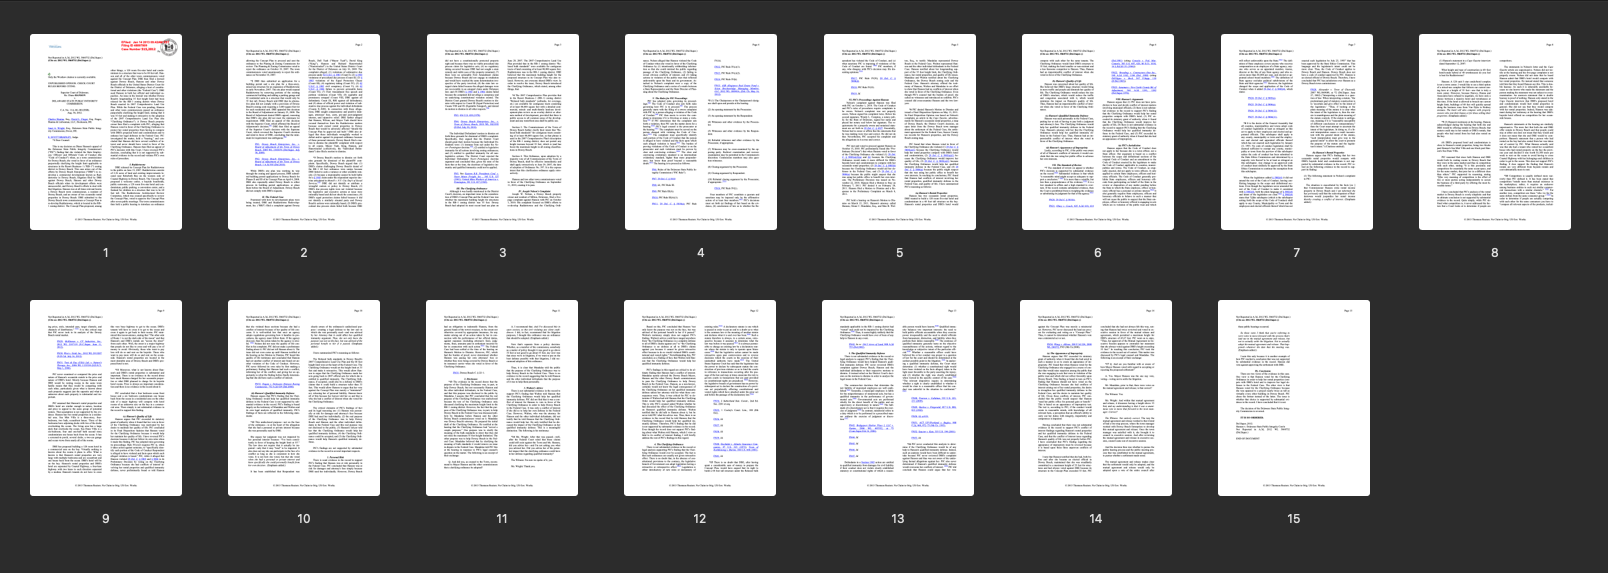
\includegraphics[width=0.95\linewidth]{figures/industrial_administration_documents.png}
    \caption{Document example about \textbf{Administration \& Industrial File}}
    \label{fig:enter-label}
\end{figure}

\begin{figure}[!htbp]
    \centering
    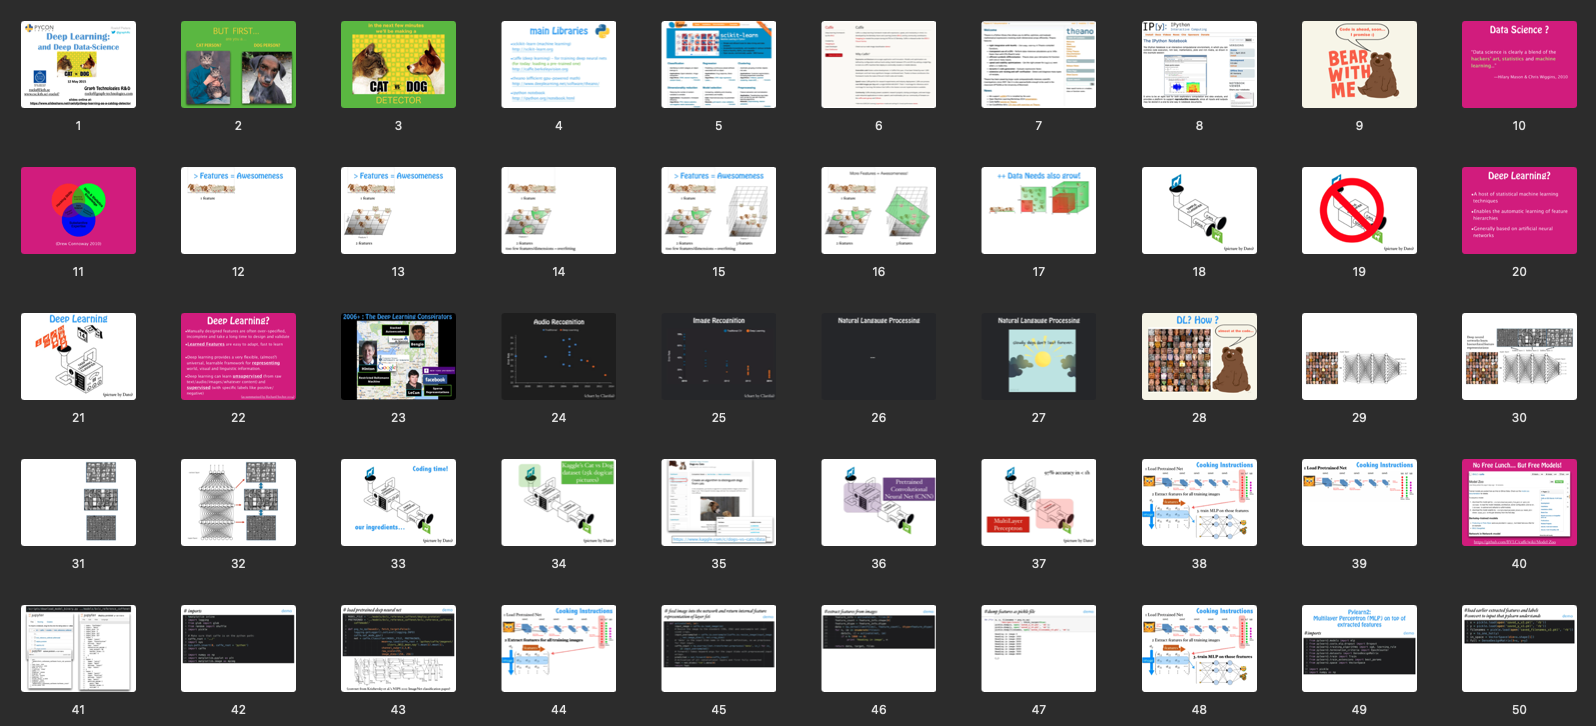
\includegraphics[width=0.95\linewidth]{figures/tutorial.png}
    \caption{Document example about \textbf{Tutorial \& Workshop} (only show first 50 pages)}
    \label{fig:enter-label_t}
\end{figure}

\begin{figure}[!htbp]
    \centering
    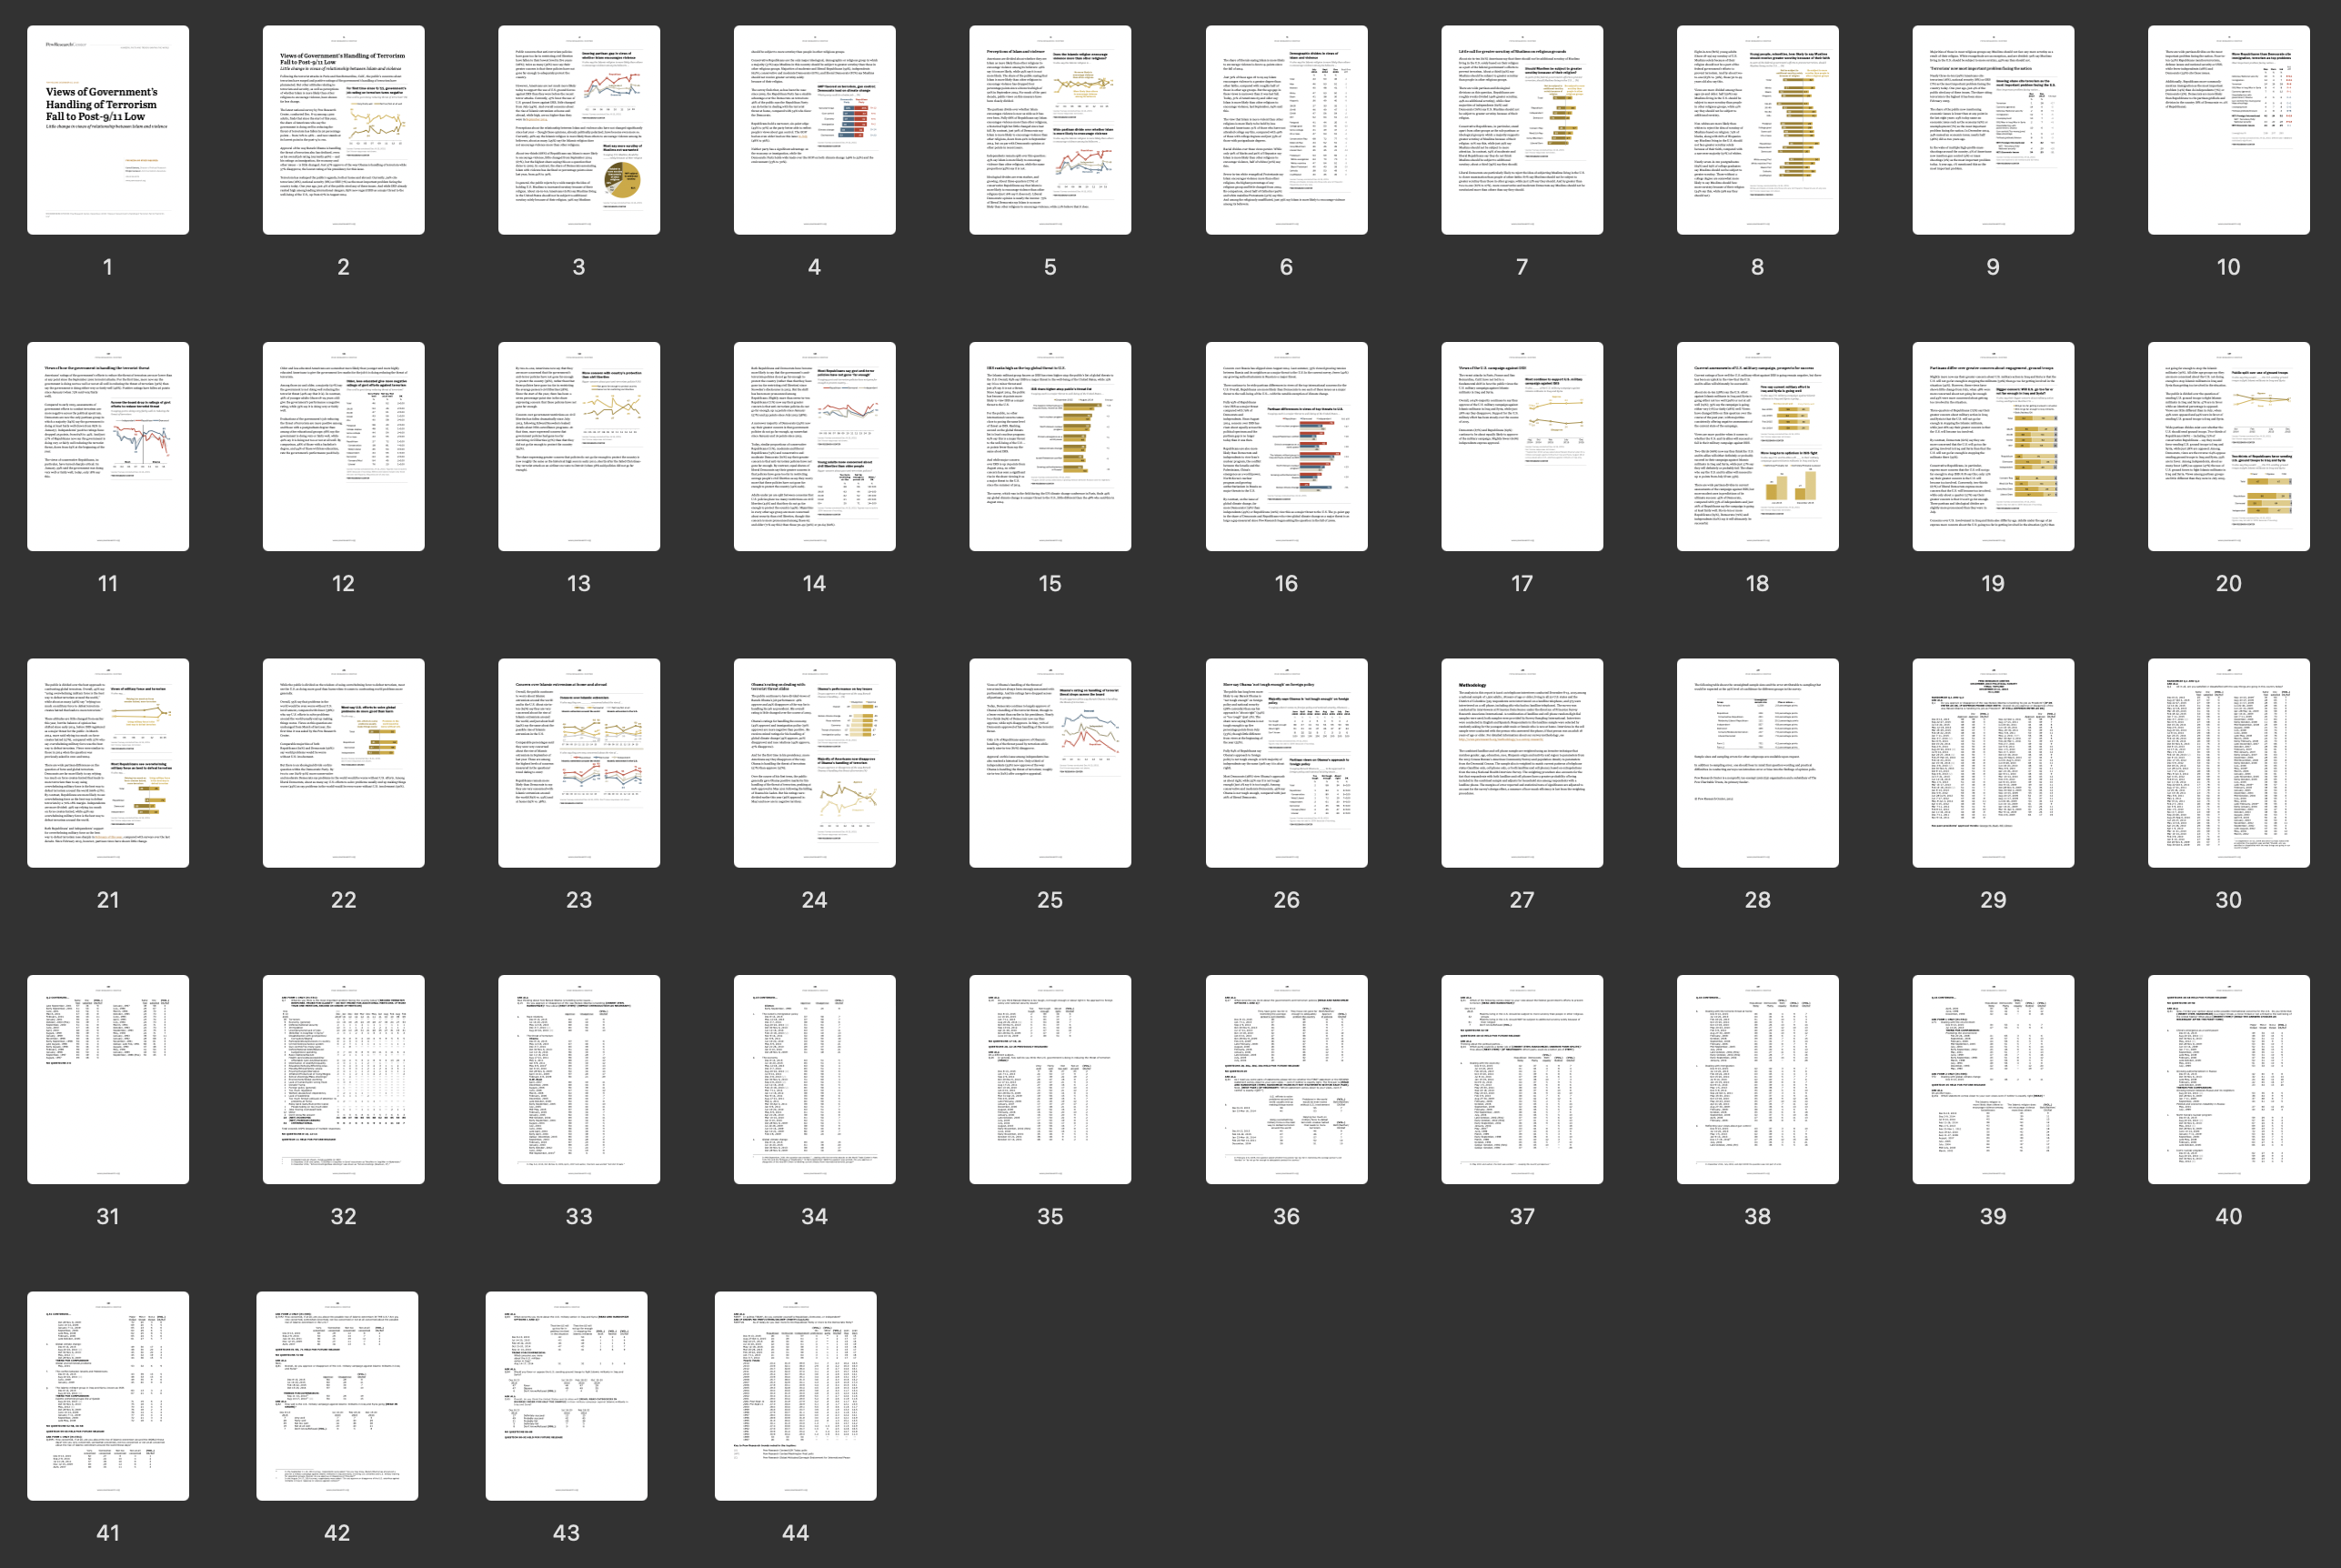
\includegraphics[width=0.95\linewidth]{figures/research_report.png}
    \caption{Document example about \textbf{Research Report}}
    \label{fig:enter-label_r}
\end{figure}

\begin{figure}[!htbp]
    \centering
    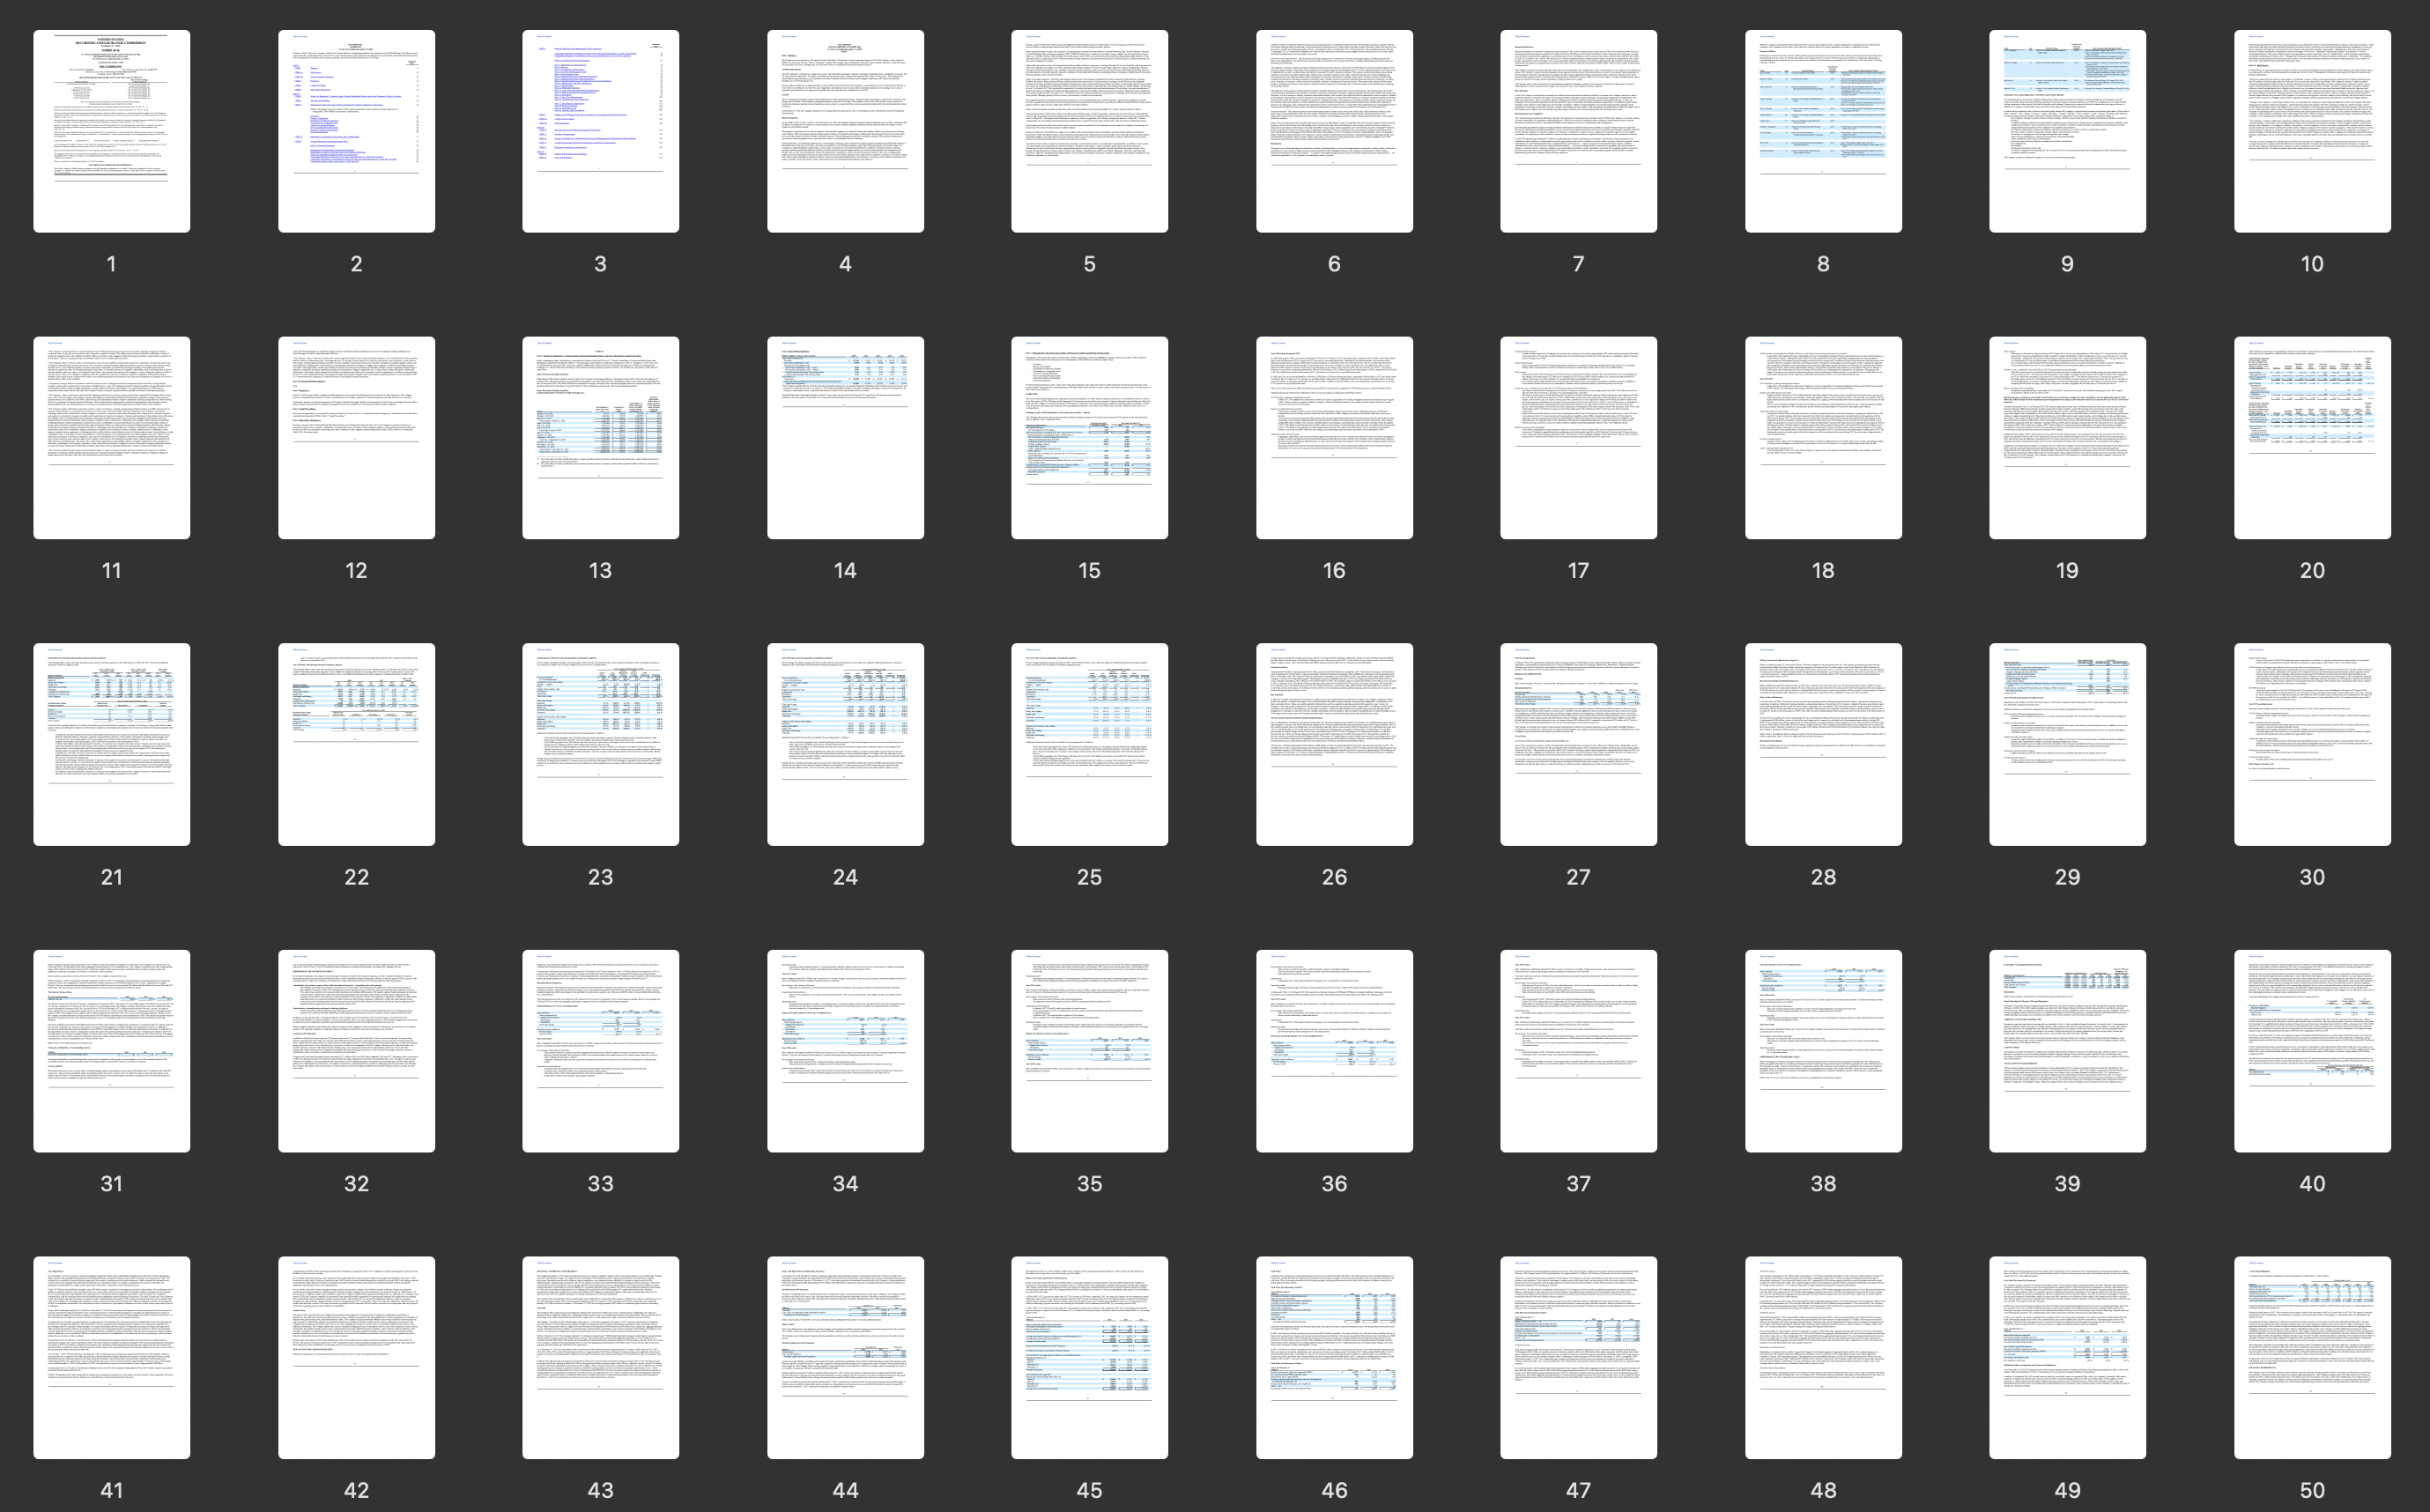
\includegraphics[width=0.95\linewidth]{figures/finance_report.png}
    \caption{Document example about \textbf{Financial Report} (only show first 50 pages)}
    \label{fig:enter-label_f}
\end{figure}

\begin{figure}[!htbp]
    \centering
    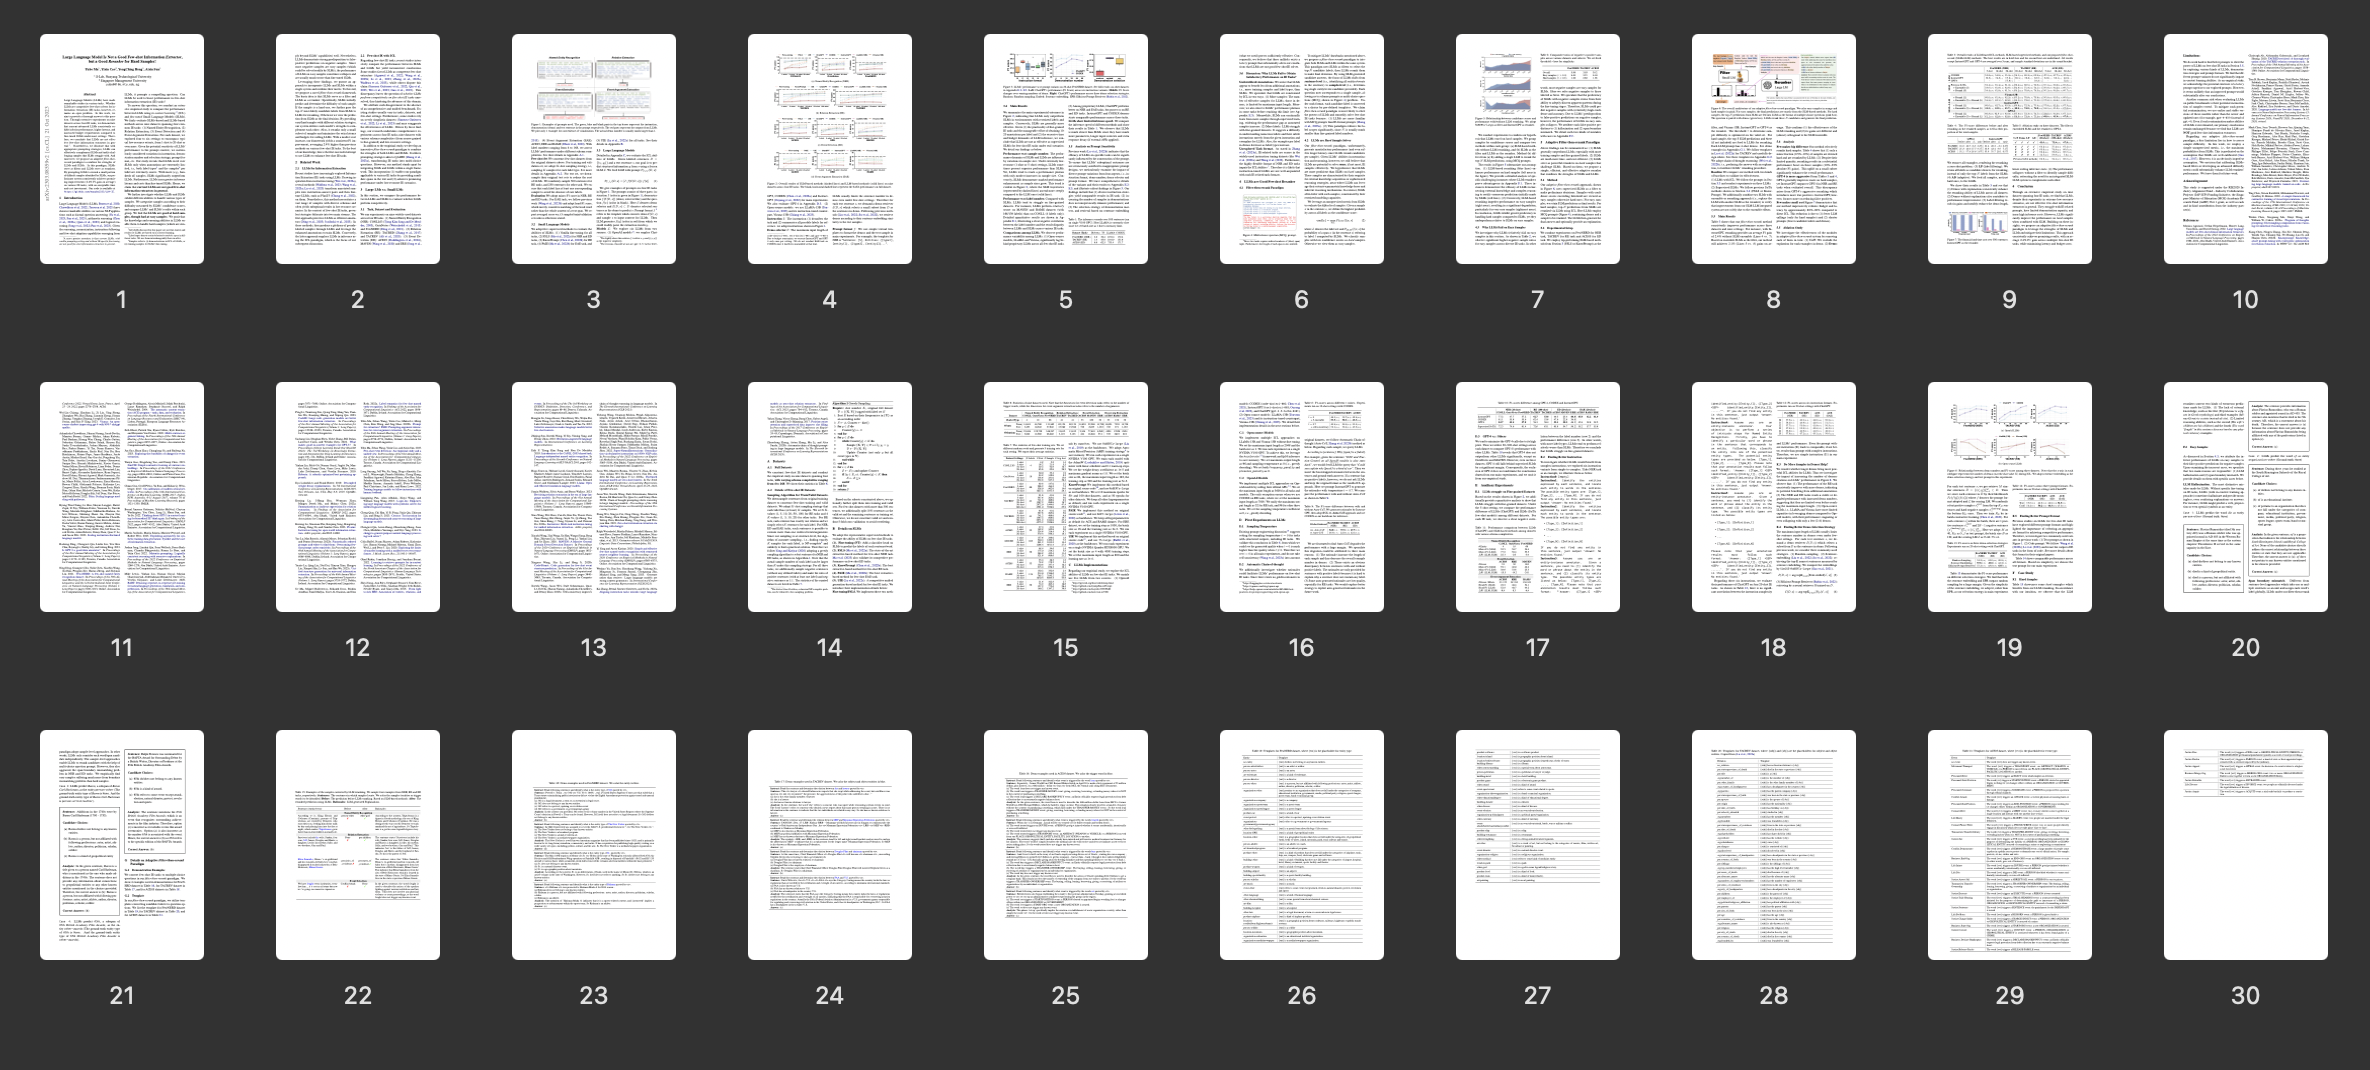
\includegraphics[width=0.95\linewidth]{figures/paper.png}
    \caption{Document example about \textbf{Academic Paper}}
    \label{fig:enter-label_a}
\end{figure}

\begin{figure}[!htbp]
    \centering
    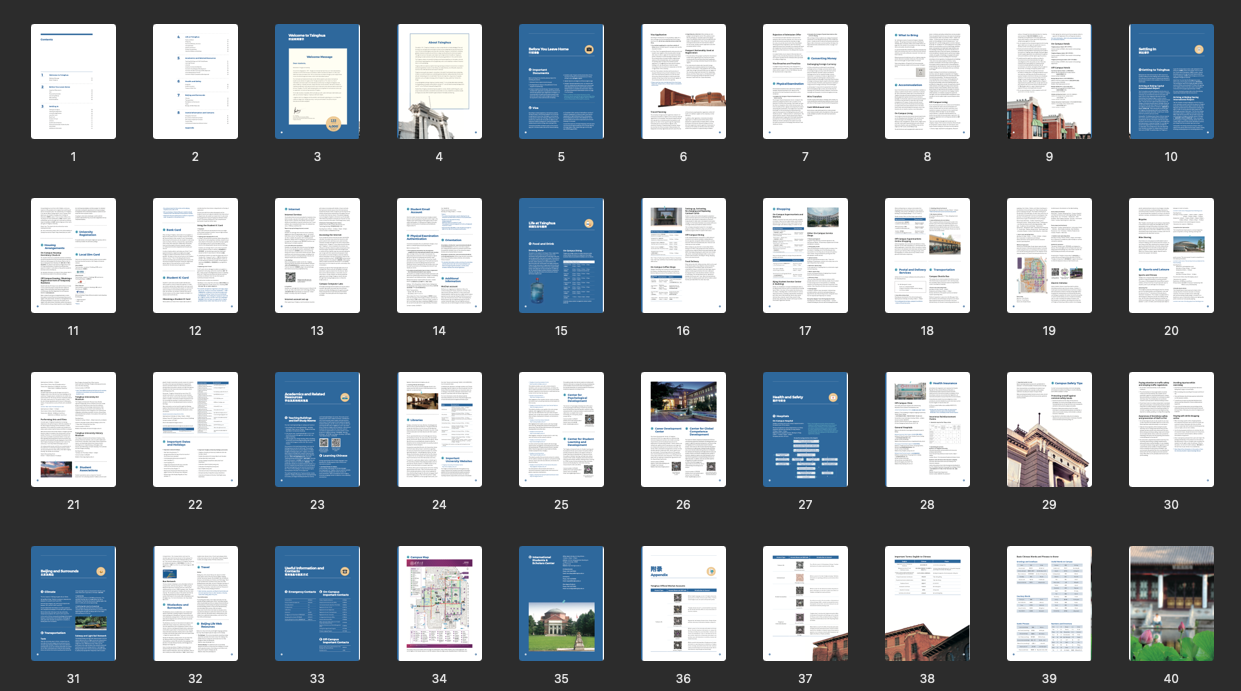
\includegraphics[width=0.95\linewidth]{figures/guideline.png}
    \caption{Document example about \textbf{Guidebook}}
    \label{fig:enter-label_g}
\end{figure}

\begin{figure}[!htbp]
    \centering
    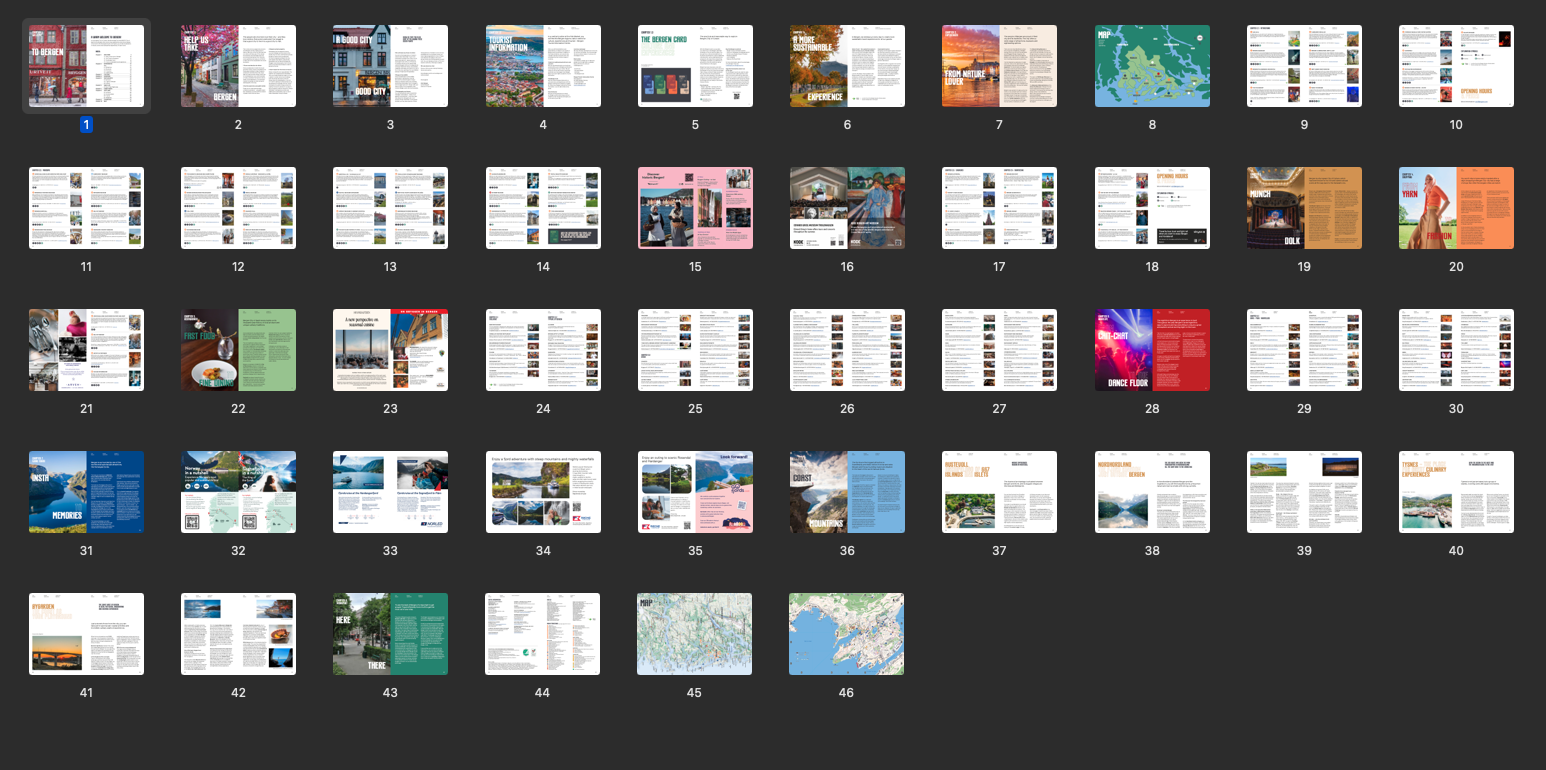
\includegraphics[width=0.95\linewidth]{figures/brochure.png}
    \caption{Document example about \textbf{Brochure}}
    \label{fig:enter-label_b}
\end{figure}

\newpage
\subsection{Existing Question Editing}
\label{subsec: Existing Question Editing}
Documents collected from existing datasets had been annotated with some questions and answers. However, their crowd-sourcing annotations inevitably make some questions, answers, and other meta information unqualified. So we conduct a systematic and manual pipeline to edit their annotations. Specifically, we classify six potential problems in original annotations. The definitions and examples of these problems are shown below.

\noindent\textbf{1. Wrong Answer or Evidence Pages:} The reference answers and/or evidence pages in original datasets are wrongly annotated.

\begin{figure}[!htbp]
    \centering
    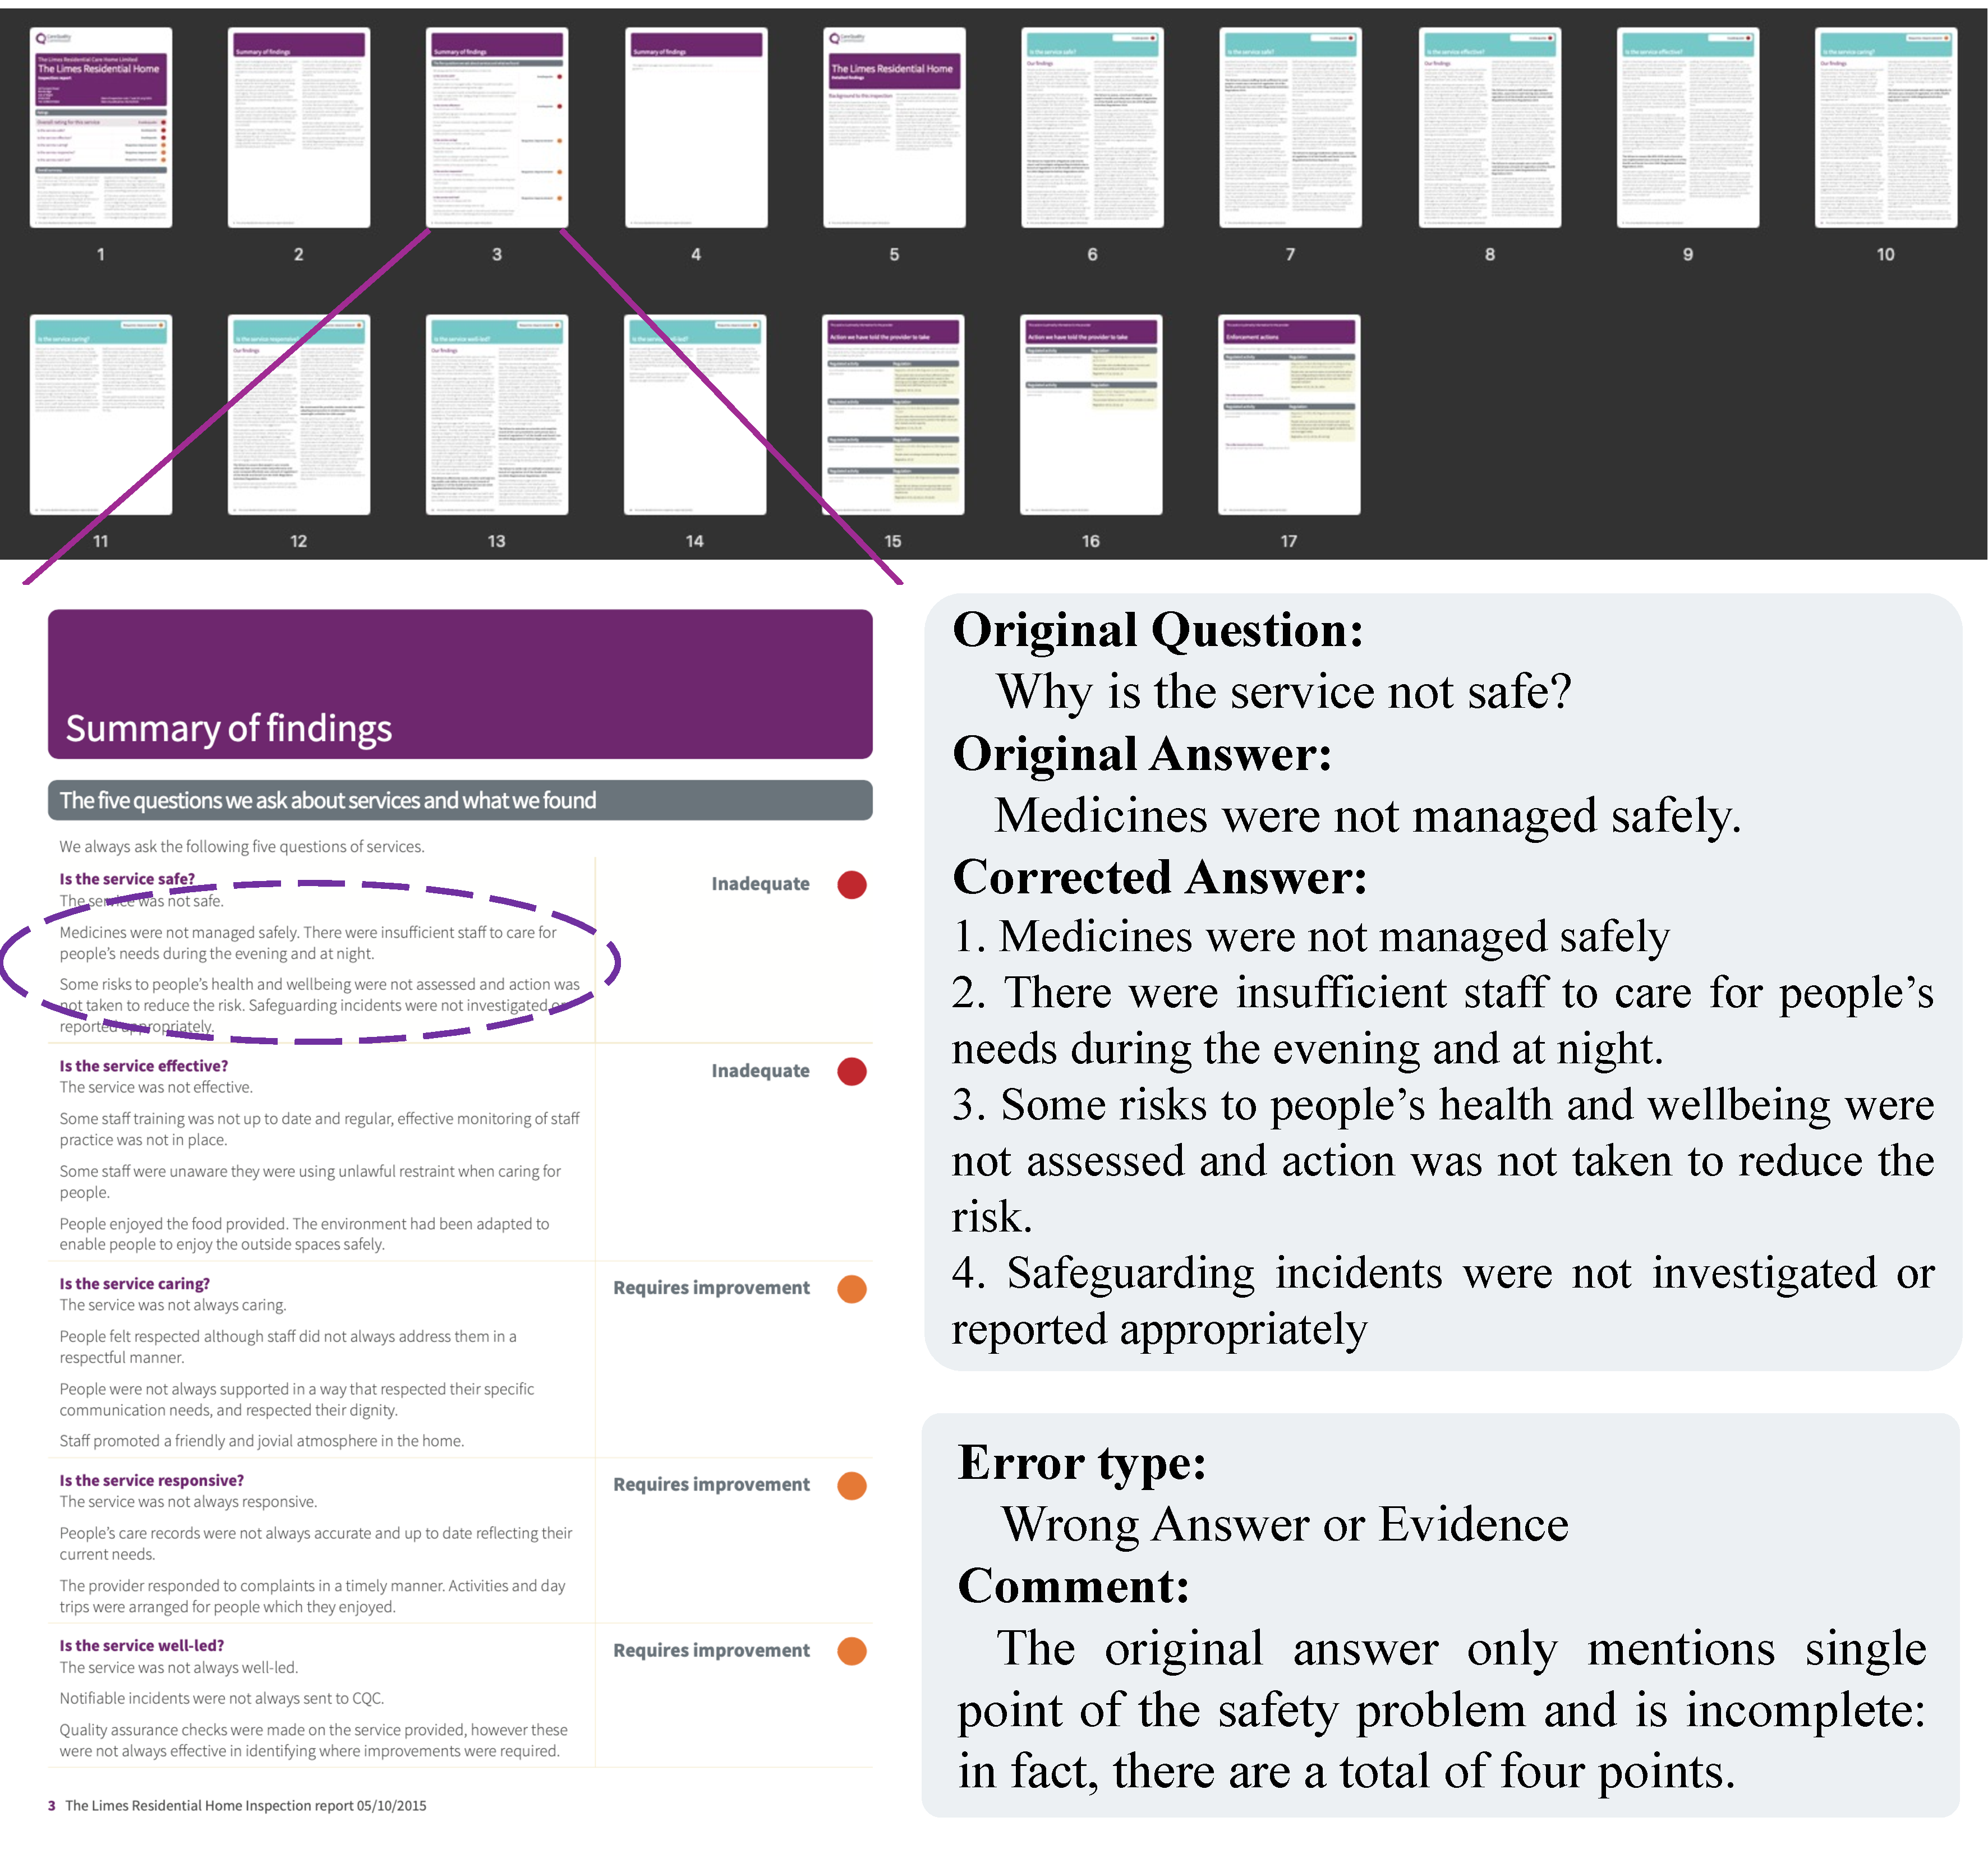
\includegraphics[width=0.95\linewidth]{figures/wrong_answers.pdf}
    \caption{Example of the original annotation with \textit{Wrong Answer or Evidence Pages}.}
    \label{fig:enter-label_e}
\end{figure}

\clearpage
\noindent\textbf{2. Repetitive Question:} Too many questions with the same types (\eg key information extraction) occur in a single document (or even on the same page or point).
 
\begin{figure}[!htbp]
    \centering
    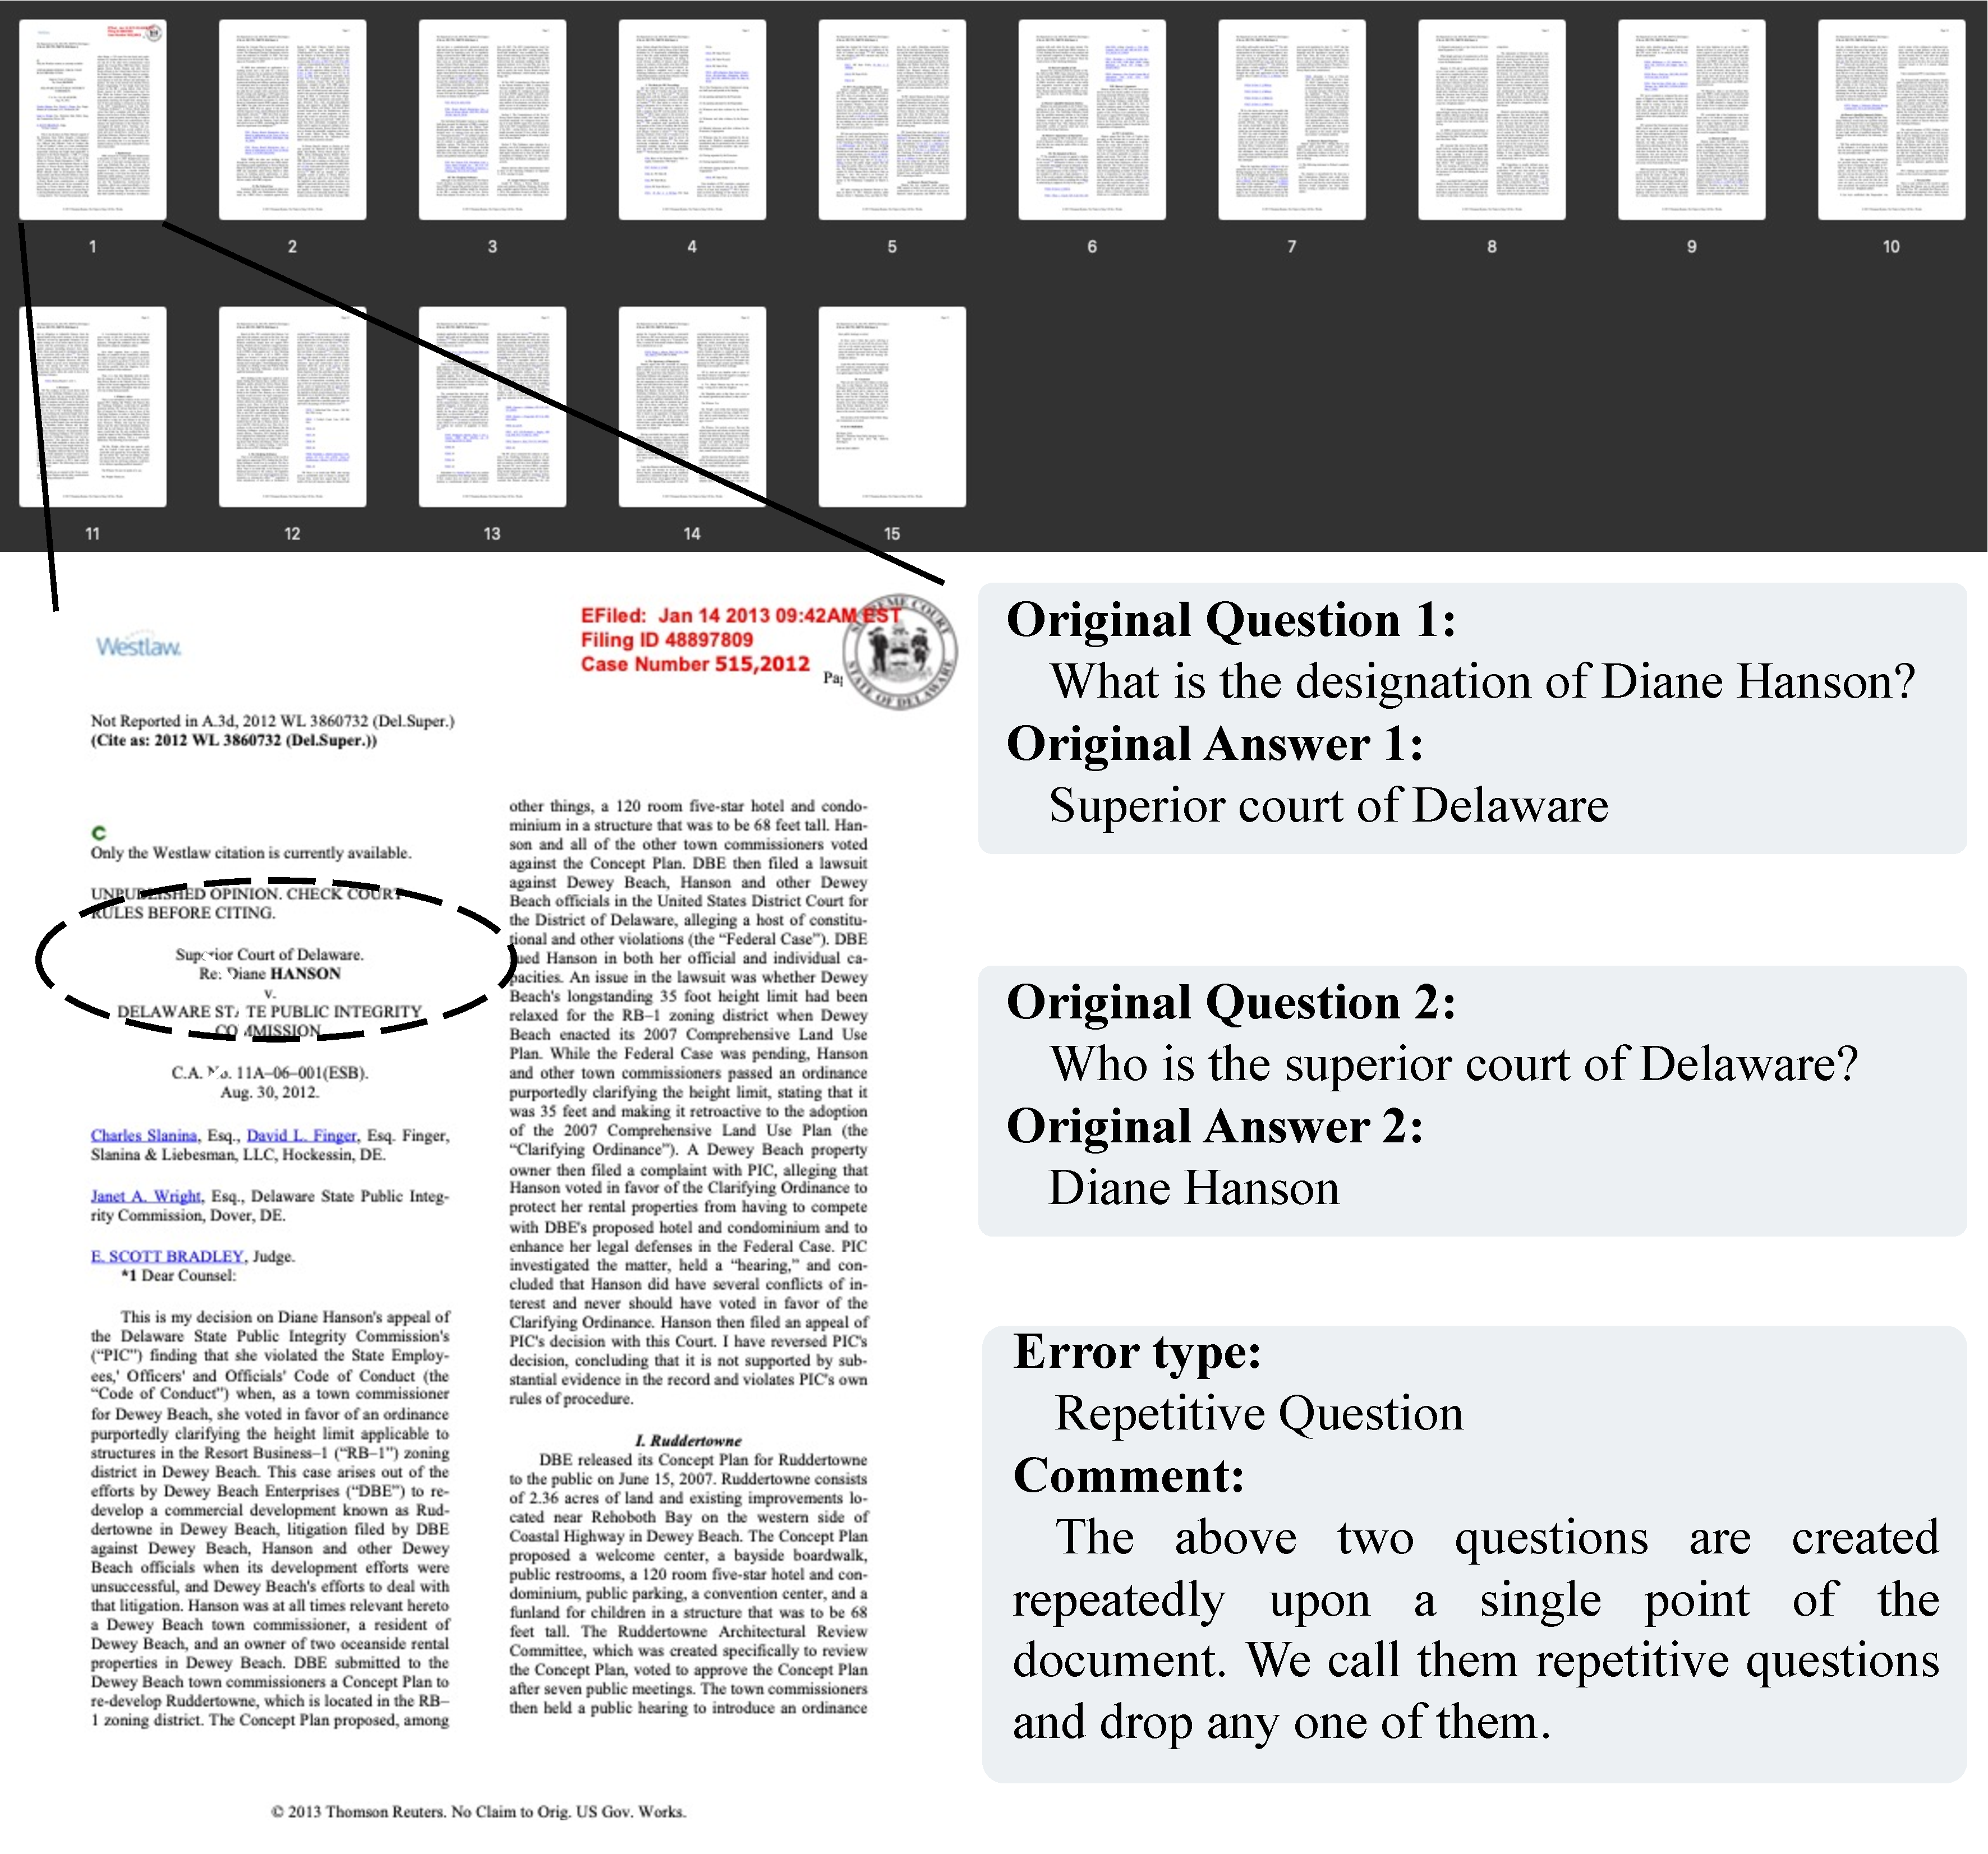
\includegraphics[width=0.95\linewidth]{figures/repetitive_question.pdf}
    \caption{Example of the original annotation with \textit{Repetitive Question}.}
    \label{fig:enter-label_q}
\end{figure}


\clearpage
\noindent\textbf{3. Ambiguous Question:} The question is ambiguous at the document level (\eg the absence of entity, period, exact section or page, \etc), or too broad to exactly answer.

\begin{figure}[!htbp]
    \centering
    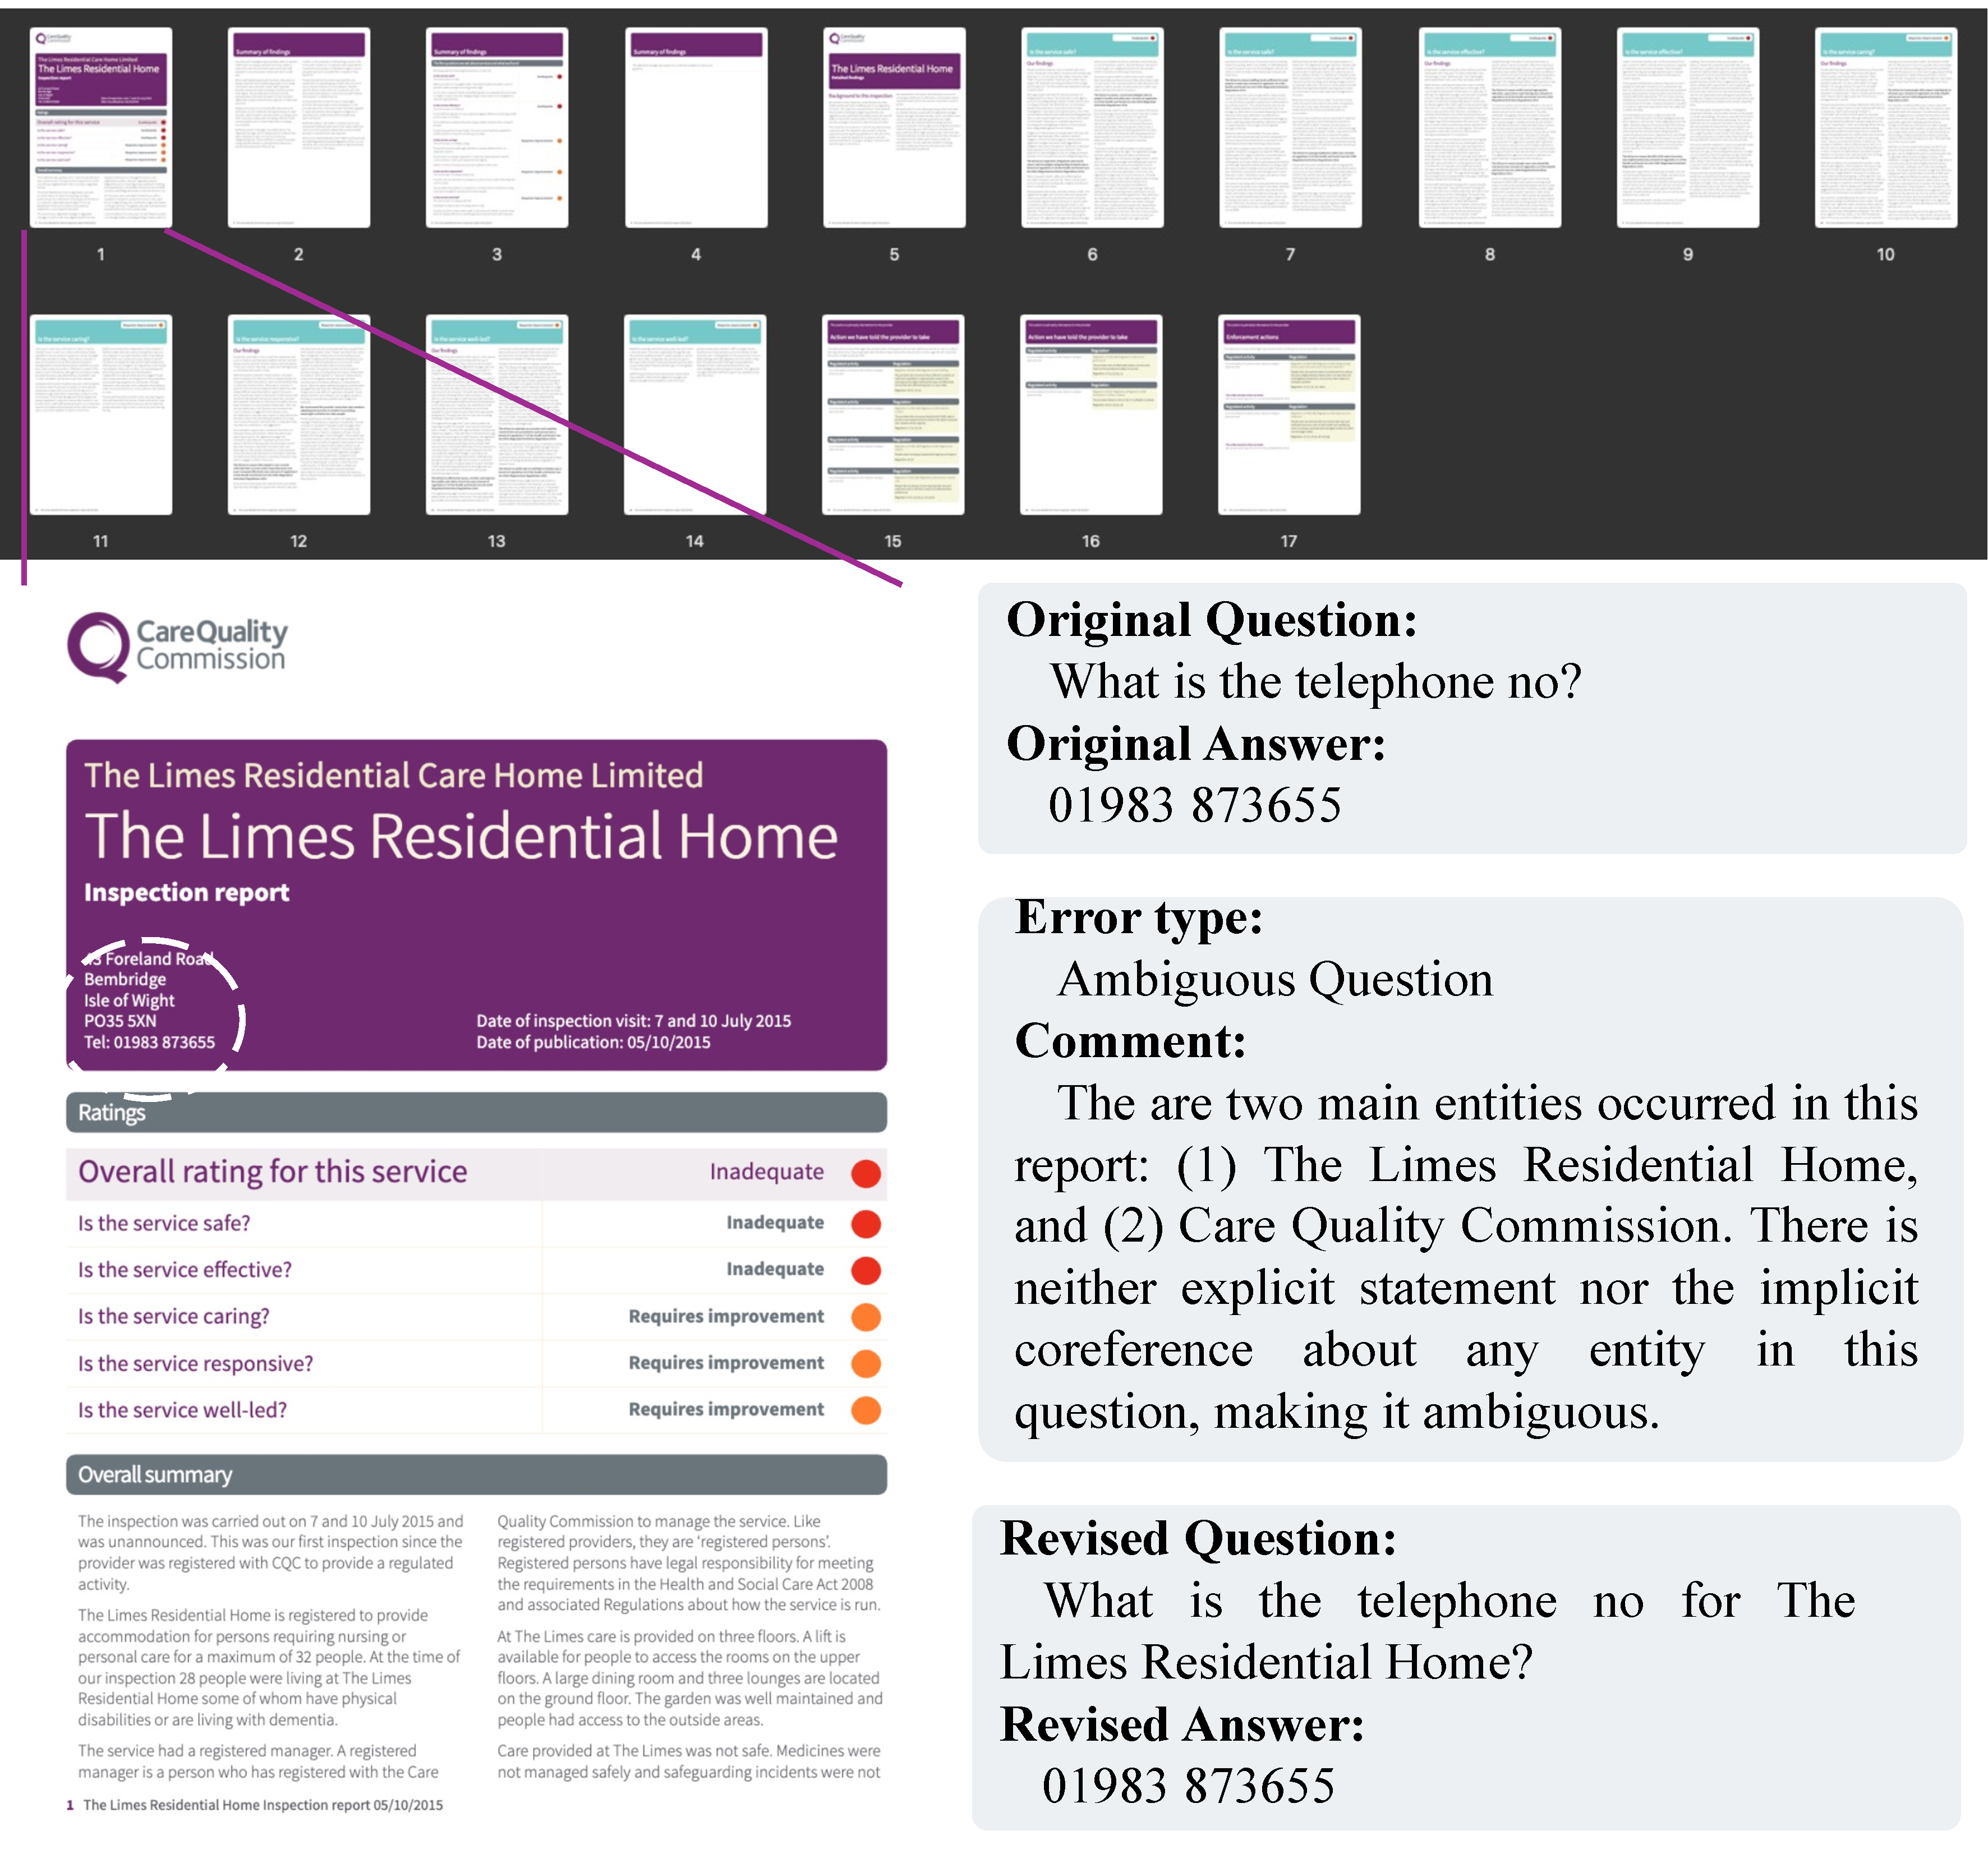
\includegraphics[width=0.95\linewidth]{figures/ambiguous_question.pdf}
    \caption{Example of the original annotation with \textit{Ambiguous Question}.}
    \label{fig:enter-label_o}
\end{figure}


\clearpage
\noindent\textbf{4. Potential Shortcut:} The resolution of the question does not rely on two entities (across different pages) but only one of them, \ie there exists a shortcut for this question.

\begin{figure}[!htbp]
    \centering
    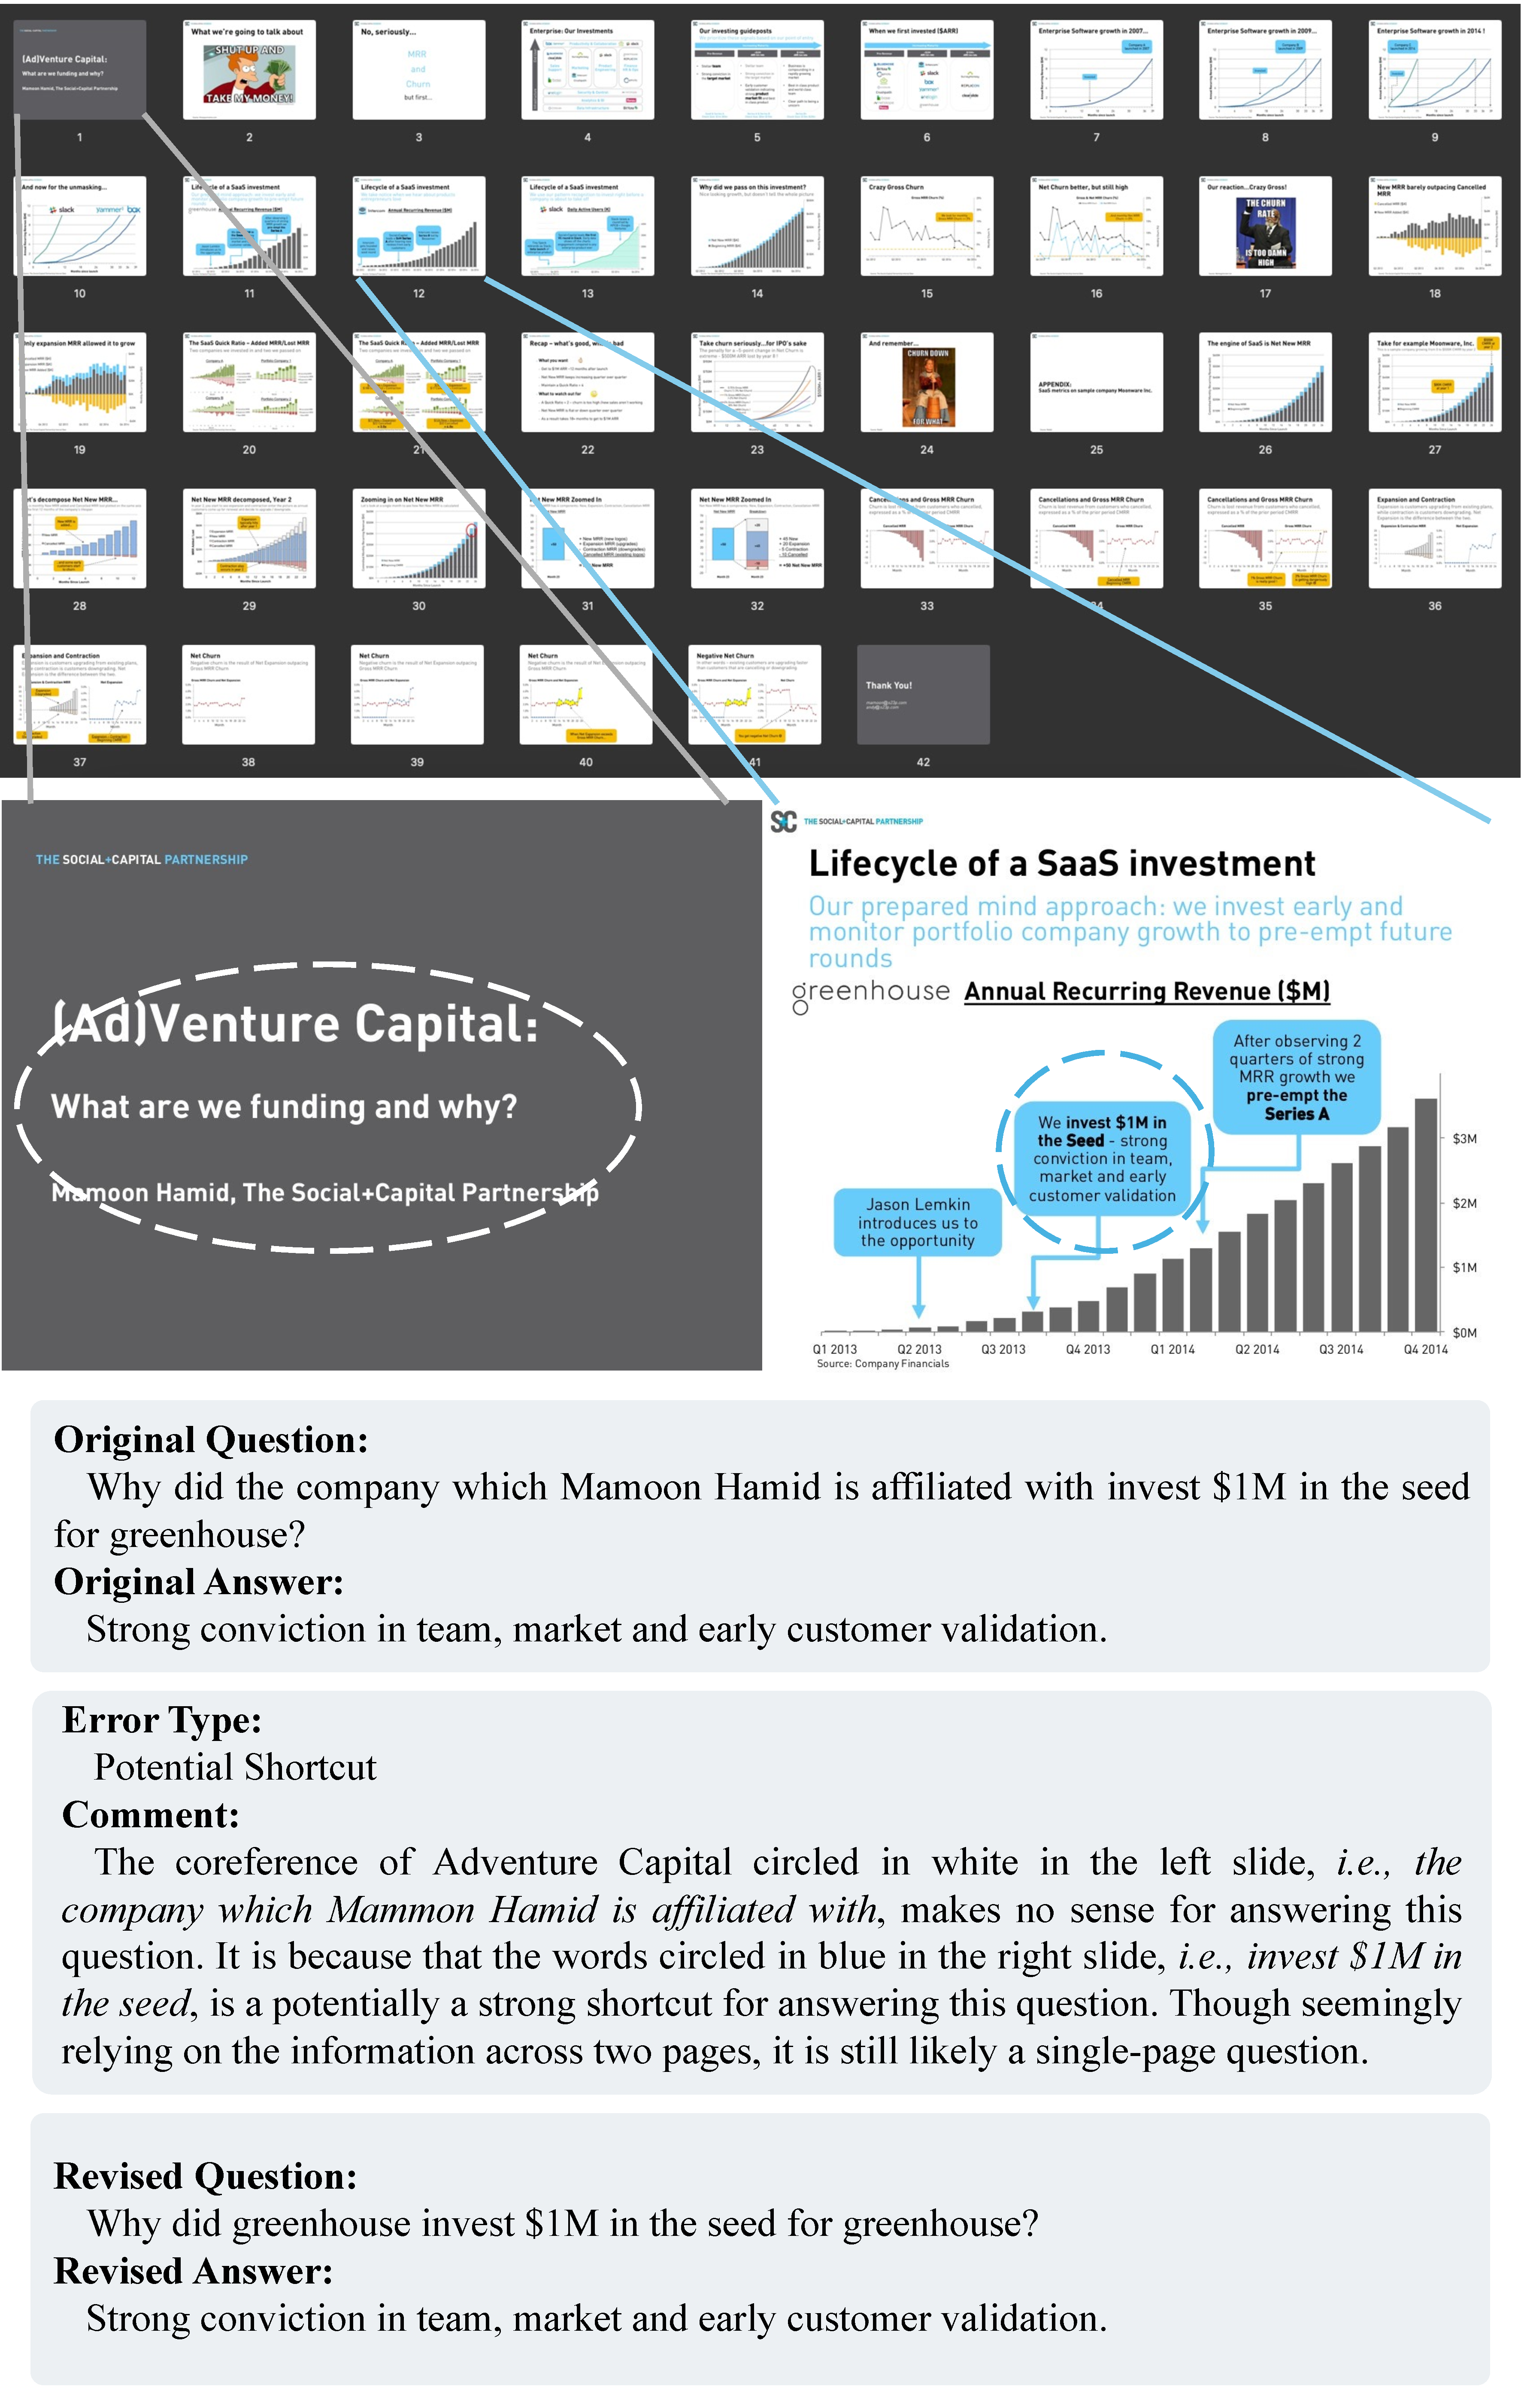
\includegraphics[width=0.92\linewidth]{figures/potential_shortcut.pdf}
    \caption{Example of the original annotation with \textit{Potential Shortcut}.}
    \label{fig:enter-label_oa}
\end{figure}


\clearpage
\noindent\textbf{5. Low Document-relevant Question:} The resolution of the question does not rely on the information from the document. It can be solved by the parametric knowledge in the LVLMs.

\begin{figure}[!htbp]
    \centering
    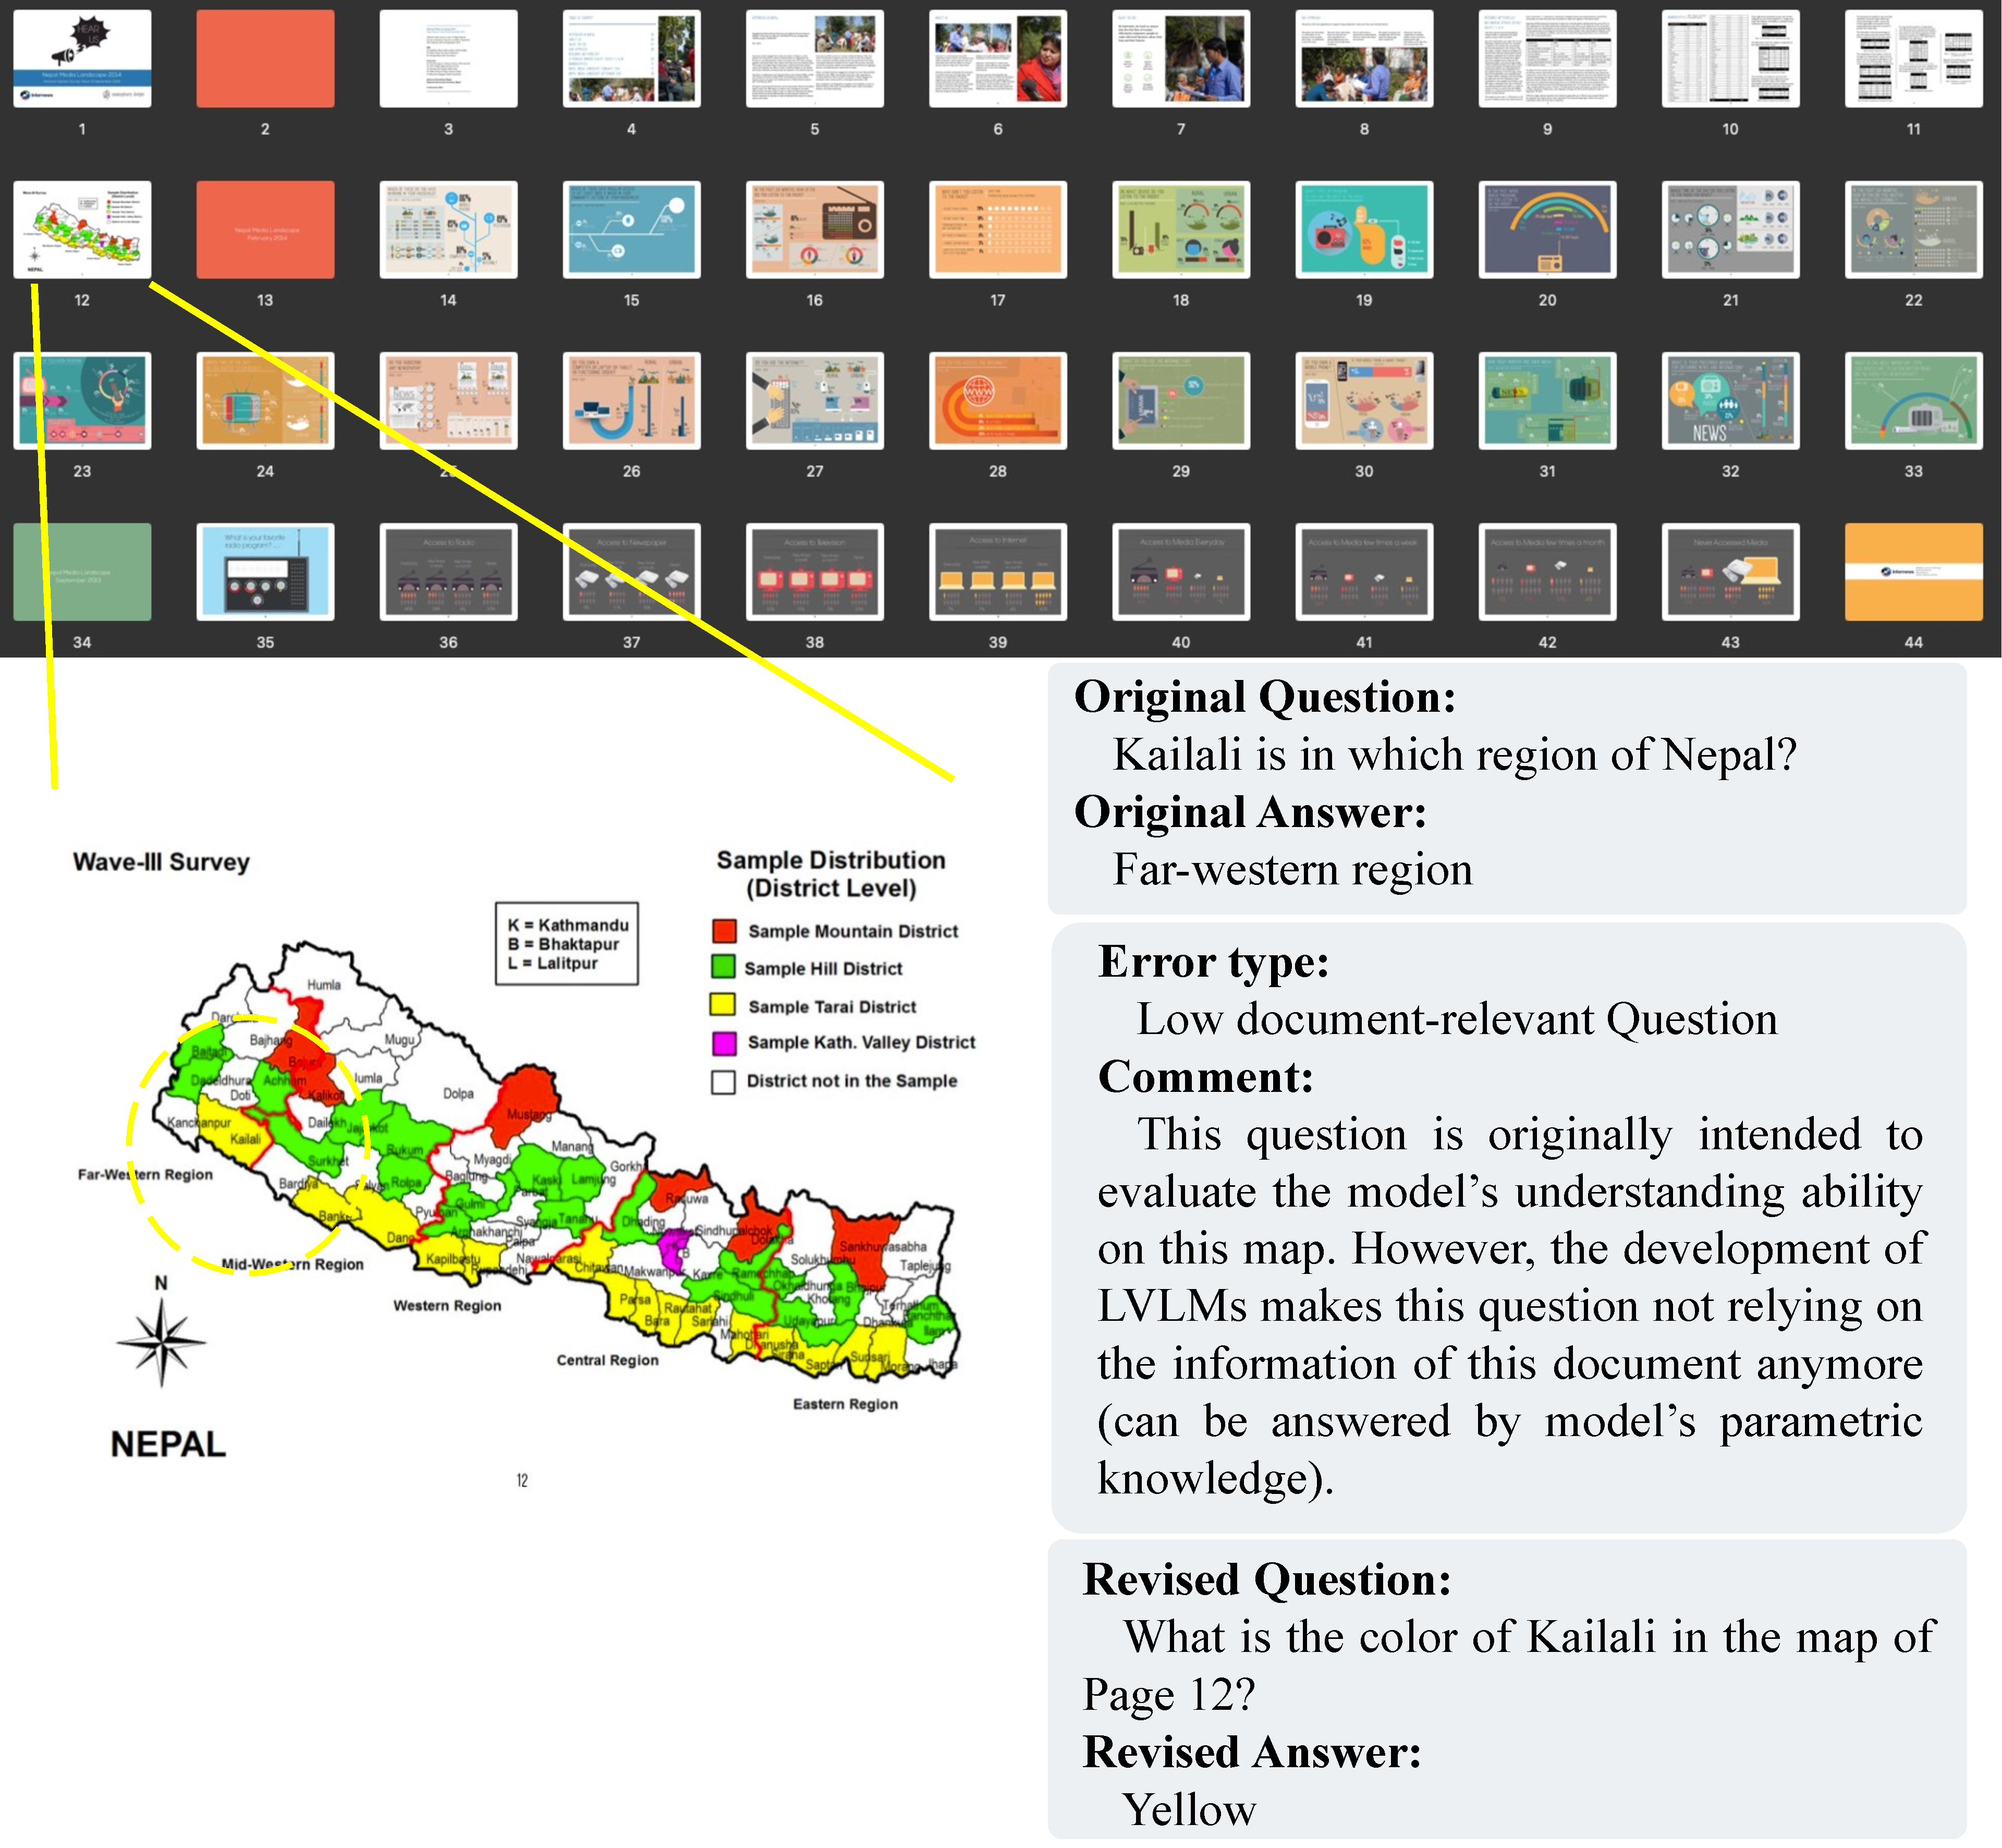
\includegraphics[width=0.95\linewidth]{figures/low_doc_relevance.pdf}
    \caption{Example of the original annotation with \textit{Low Document-relevant Question}.}
    \label{fig:enter-label_l}
\end{figure}

\clearpage
\noindent\textbf{6. Decontextulization-required Question:} The understanding of the question is conditioned on a single page or even a single component of the document.

\begin{figure}[!htbp]
    \centering
    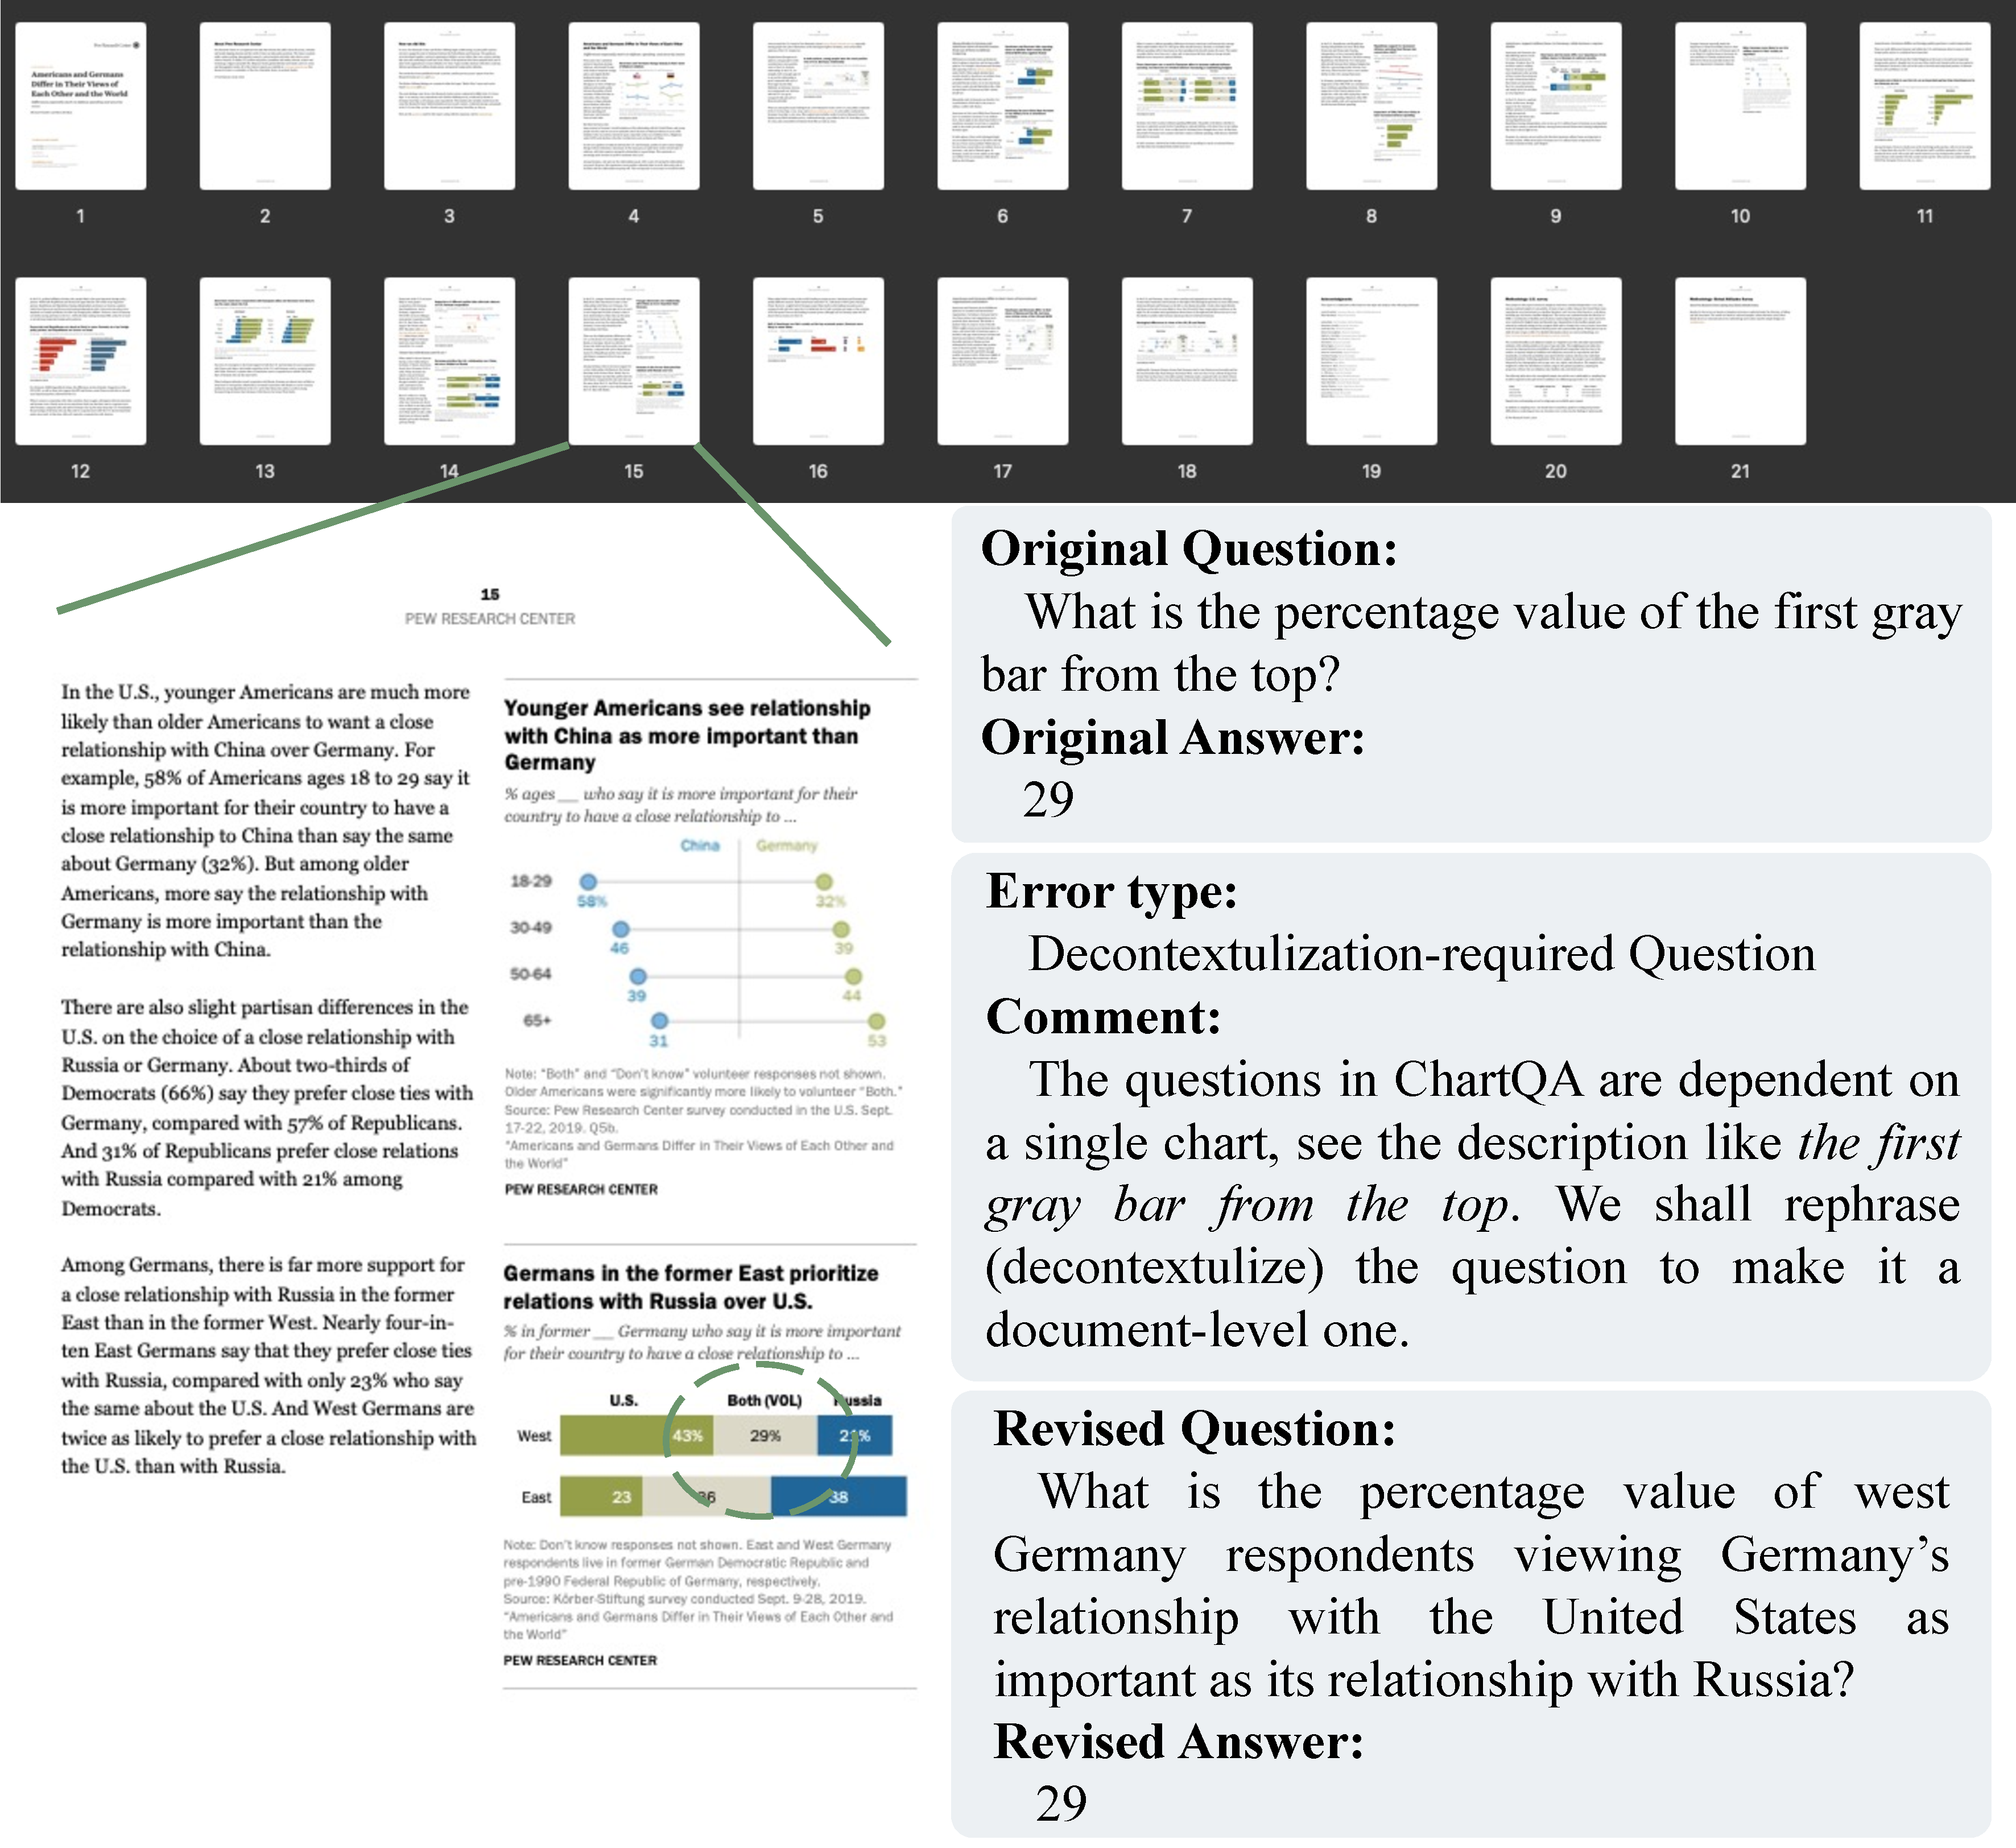
\includegraphics[width=0.95\linewidth]{figures/decontextulization_question.pdf}
    \caption{Example of the original annotation with \textit{Decontextulization-required Question}.}
    \label{fig:enter-label_dr}
\end{figure}


When dealing with questions categorized under any of these six problem types, annotators are instructed to either revise or remove them. Typically, repetitive questions and those with potential shortcuts are removed. In contrast, wrongly-annotated or decontextualization-required questions are generally revised. For ambiguous and low document-relevant questions, the course of action depends more on the annotators' discretion.

\clearpage
\subsection{New Question Annotation}
\label{appendix: New Question Annotation}
We annotate new questions on both existing and newly-collected documents. To ensure a diverse range of questions, we impose limitations on the question distributions categorized by their types (\ie single-page, cross-page or unanswerable) and evidence sources (\ie table, chart, image). To balance existing questions which are mostly single-page and text-based, we place greater emphasis on cross-page, unanswerable, table-related, chart-related, and image-related questions. The detailed standards are as follows:

\begin{table}[!htbp]
    \centering
        \begin{tabular}{l|cc|ccc|c}
        \toprule
        \multirow{2}{*}{\textbf{Document Type}}  &  \multicolumn{2}{c}{\textbf{Evidence Page}}  & \multicolumn{3}{c}{\textbf{Evidence Source}} & \multirow{2}{*}{\textbf{All}} \\
        & Cross-page & Unanswerable & Table & Chart & Image \\
        \midrule
        Industrial File & $\geq 2$ & - & \multicolumn{3}{c}{-} \vline & $\geq 3$ \\
        Workshop \& Tutorial & $\geq 2$  & $\geq 1$ & \multicolumn{3}{c}{------ $\geq 3$ ------} \vline & $\geq 6$  \\
        Research Report &  $\geq 3$ & $\geq 1$ & $\geq 2$ & $\geq 2$ & - & $\geq 5$ \\
        Financial Report &  $\geq 5$ & $\geq 2$ & $\geq 7$ & - & - & $\geq 10$ \\
        Academic Paper &  $\geq 3$ & $\geq 1$ & $\geq 2$ & \multicolumn{2}{c}{---- $\geq 3$ ----} \vline & $\geq 6$ \\
        Guidebook & $\geq 3$ & $\geq 1$ & -& - & $\geq 4$ & $\geq 7$ \\ 
        Brochure & $\geq 2$ & $\geq 1$ & -& - & $\geq 3$ & $\geq 7$ \\
        \bottomrule
        \end{tabular}
    \vspace{0.5em}
    \caption{The \textbf{minimum} requirements for the number and distribution of questions, categorized by the evidence page numbers and evidence sources. We have set varying requirements for different document types based on their specific characteristics.}
    \label{tab:my_label}
\end{table}

\subsection{Potential Bias for LVLM-based Quality Checking}
\label{appendix: potential_bias}
As described in Section~\ref{subsec: quality control}, we employ GPT-4o to remove document-agnostic (\ie can be correctly answer without documents) samples and review potential wrongly-labeled samples. A reasonable speculation raises that our final benchmark can be biased toward GPT-4o’s answers, especially when GPT-4o outperforms others by a large margin. We discuss this potential bias as follows. 

We check the effect of GPT-4o's involvement in the quality control step-by-step. Specifically, we compare the performance of samples remained after each step across GPT-4o and two other competitive models (GPT-4V and Gemini-1.5-Pro). We show their results in the table below.

\begin{table}[!htbp]
    \centering
    \resizebox{0.95\linewidth}{!}{
    \begin{tabular}{l|ccc}
    \toprule
        & \textbf{GPT-4o} & \textbf{GPT-4V} & \textbf{Gemini-1.5-Pro} \\
         \midrule
        No quality control & 43.1\% & 35.2\%  & 23.3\%  \\
        \quad + document-relevance detection & 41.2\%  & 31.0\%  & 20.5\%  \\
        \quad + document-relevance detection + self-reflection / cross-checking & 42.7\%  & 31.4\%  & 20.9\%  \\
        \bottomrule
    \end{tabular}
    }
    \vspace{1em}
    \caption{Step-wise performance comparison with and without LVLM-based quality checking}
    \label{tab:perform_compare}
\end{table}

The results illustrate that the potential bias in step 1 (document-relevance detection) actually reduce, rather than increase, the performance gap between GPT4o and other models. It is because that we filter out all samples correctly answered by GPT4o without the access to documents. Under this case, the more significant performance drop of GPT-4V and Gemini-1.5-Pro can only be attributed to their limited document understanding and over-reliance on their internal knowledge. Regarding the step 2 and 3 (self-reflection and cross-checking), we provide inconsistent answers between human annotations and GPT4o's predictions to annotators and ask them to check and revise accordingly. The potential bias of this step does lead to a slight performance bias (1.1\% absolute difference at maximum). We believe that such bias is NOT the main cause of GPT4o's significantly best performance. Without the involvement of GPT-4o in the quality control process, GPT-4o still significantly outperforms GPT-4V by 7.9\% (43.1\% - 35.2\%) and Gemini-1.5-Pro by 19.8\% (43.1\% - 23.3\%). Accordingly, all primary conclusions in our paper still hold.


\clearpage
\subsection{GUI Screenshots}
\label{appendix: GUI Screenshots}
We present the screenshots for editing existing questions and annotating new questions (along with their reference answers and meta-data) in Figure~\ref{fig: GUI_existing} and Figure~\ref{fig: GUI_new} respectively.

\begin{figure}[!htbp]
    \centering
    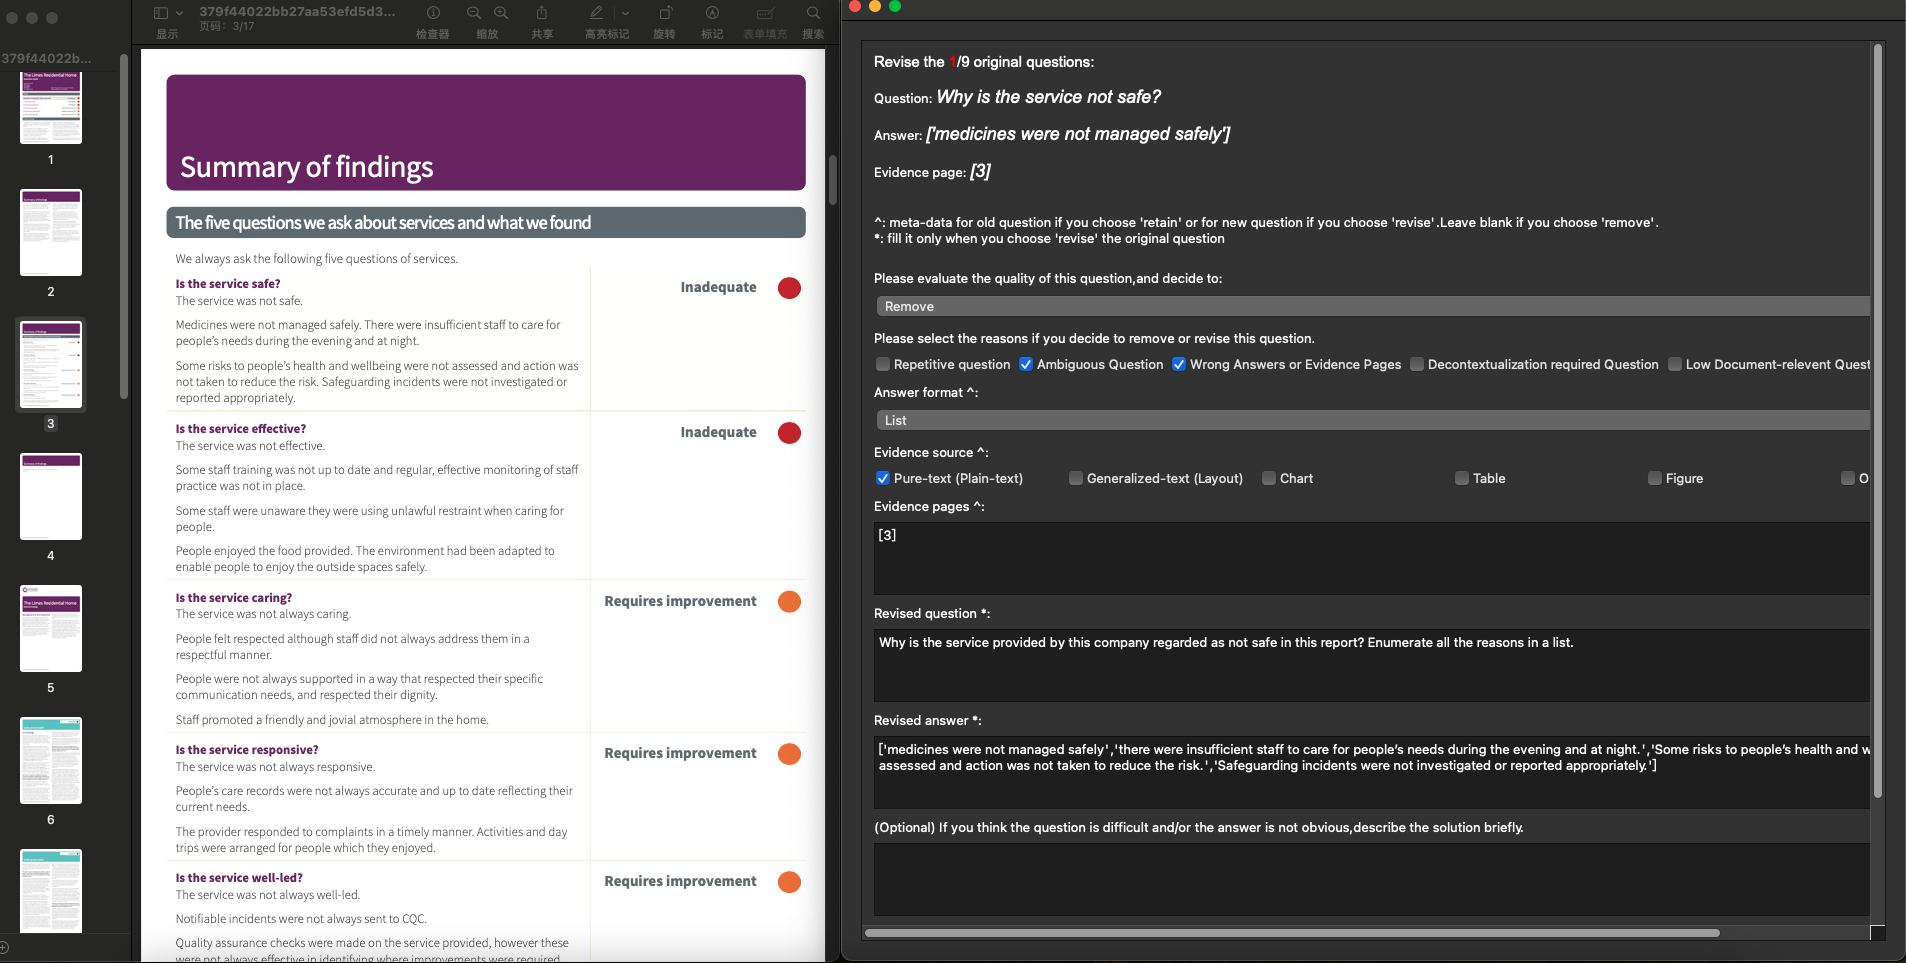
\includegraphics[width=0.95\linewidth]{figures/GUI_existing_question.png}
    \caption{GUI screenshot for editing existing questions (along with reference answers and meta-data)}
    \label{fig: GUI_existing}
\end{figure}

\begin{figure}[!htbp]
    \centering
    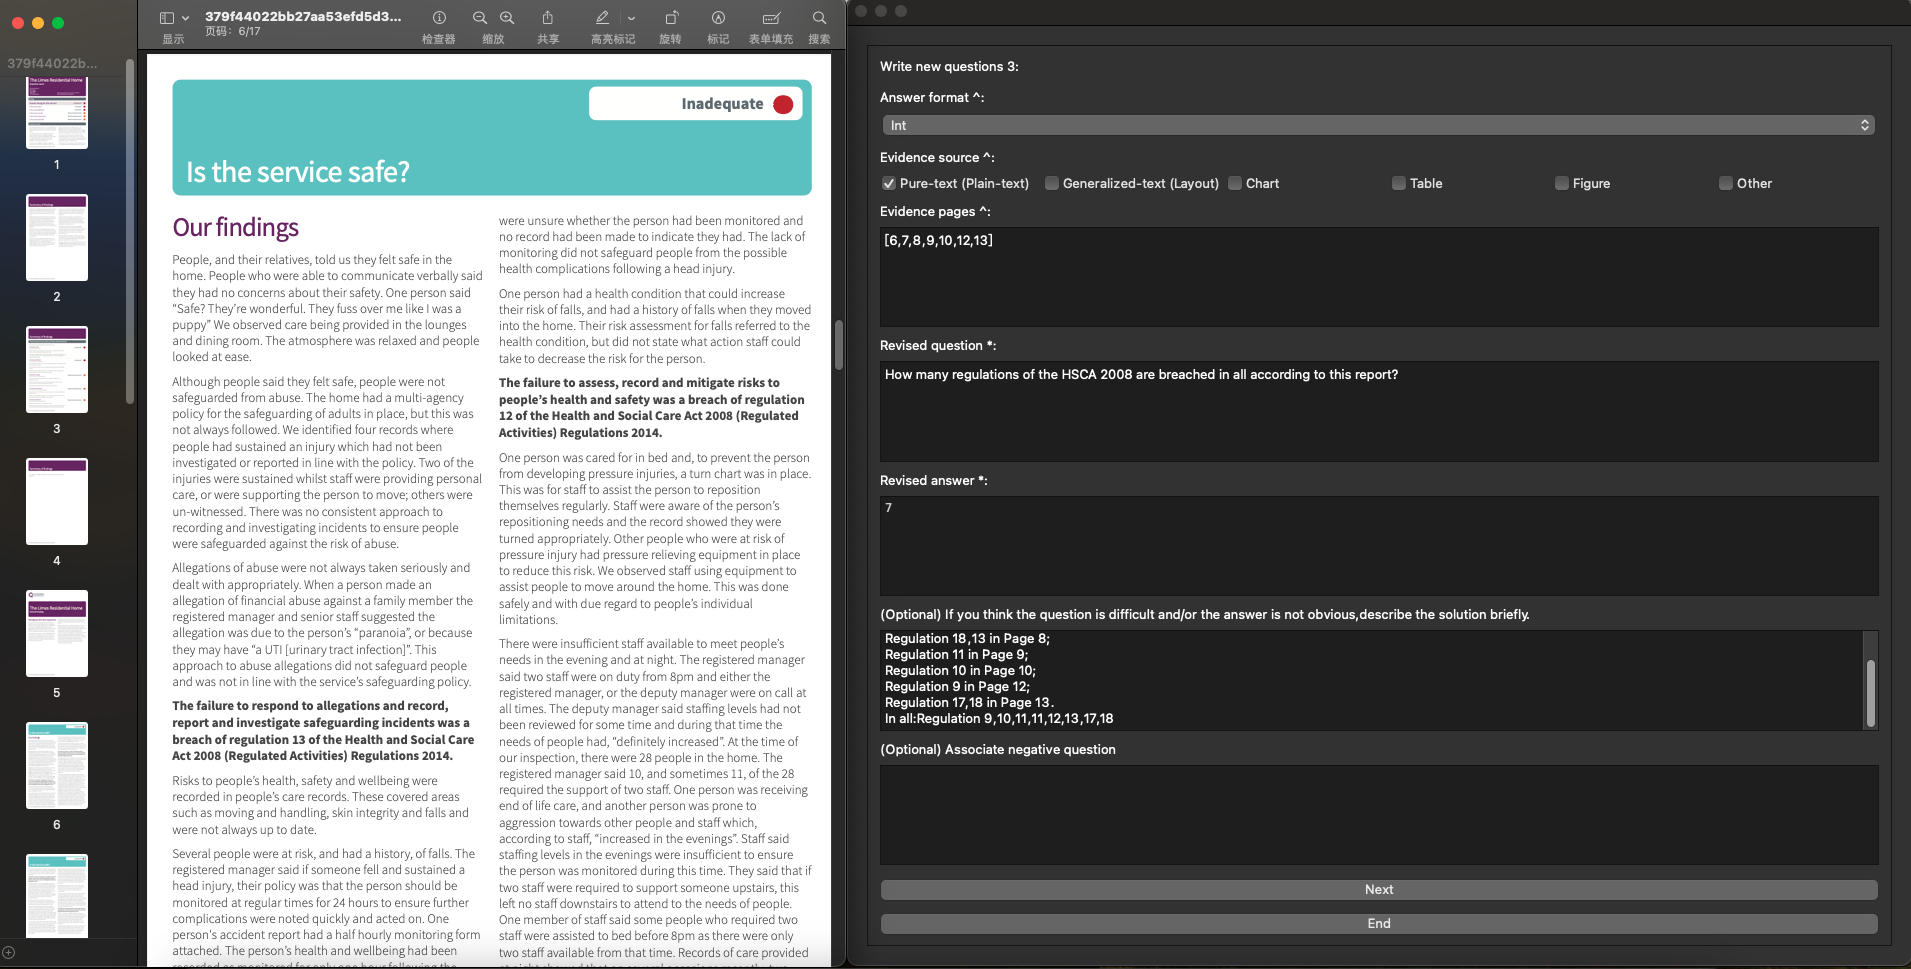
\includegraphics[width=0.95\linewidth]{figures/GUI_new_question.png}
    \caption{GUI screenshot for annotating new questions (along with reference answers and meta-data)}
    \label{fig: GUI_new}
\end{figure}

\subsection{Annotation Cost}
This benchmark is annotated by the authors of this paper. Therefore, the data collection does not need compensation. And we count the time cost of our benchmark as below.

\noindent \textbf{Pre-annotation} (about 45h): the development of annotation interface (10h), the writing of annotation guideline (5h), training session (10h), preliminary annotation and personalized feedback (20h).

\noindent \textbf{Annotation} (about 150h): It takes about 60-90 minutes for the annotation of each document. And all of the 130 documents take about 150 hours.

\noindent \textbf{Post-annotation} (about 45h): quality checking (30h), data processing and release preparation (15h).

In summary, our benchmark annotation approximately takes a total of 45+150+45=240 hours (1.36 man months).